\clearpage

In the following, we show the unfolded data distributions for the different jet algorithms under study, comapared to the MC expectations from Madgraph and Herwig++. In all distributions, the MC is normalized to the data. The distributions are integrated in the jet momentum. 

We report normalized cross-sections, i.e. $1/sigma*(d/sigma/dM_J)$ in order to cancel luminosity dependence.
The MC is found to reproduce pretty well the data, with some residual poor modeling at low mass (that is also the most sensitive region to PU effects). It is also interesting to observe that the more aggressive the grooming is, the more herwig seems to better reproduce the data than madgraph/pythia. 


\subsection{$Z(\mu\mu)$+ jet Analysis}

Fig.~\ref{figs:AK7ZmmInt1} shows the jet mass distribution for AK7 jets in Z$(\mu\mu)$ +jet events, for the different clustering algorithm studied: ungroomed, pruned, trimmed and filtered respectively.  

\begin{figure}[!htb]
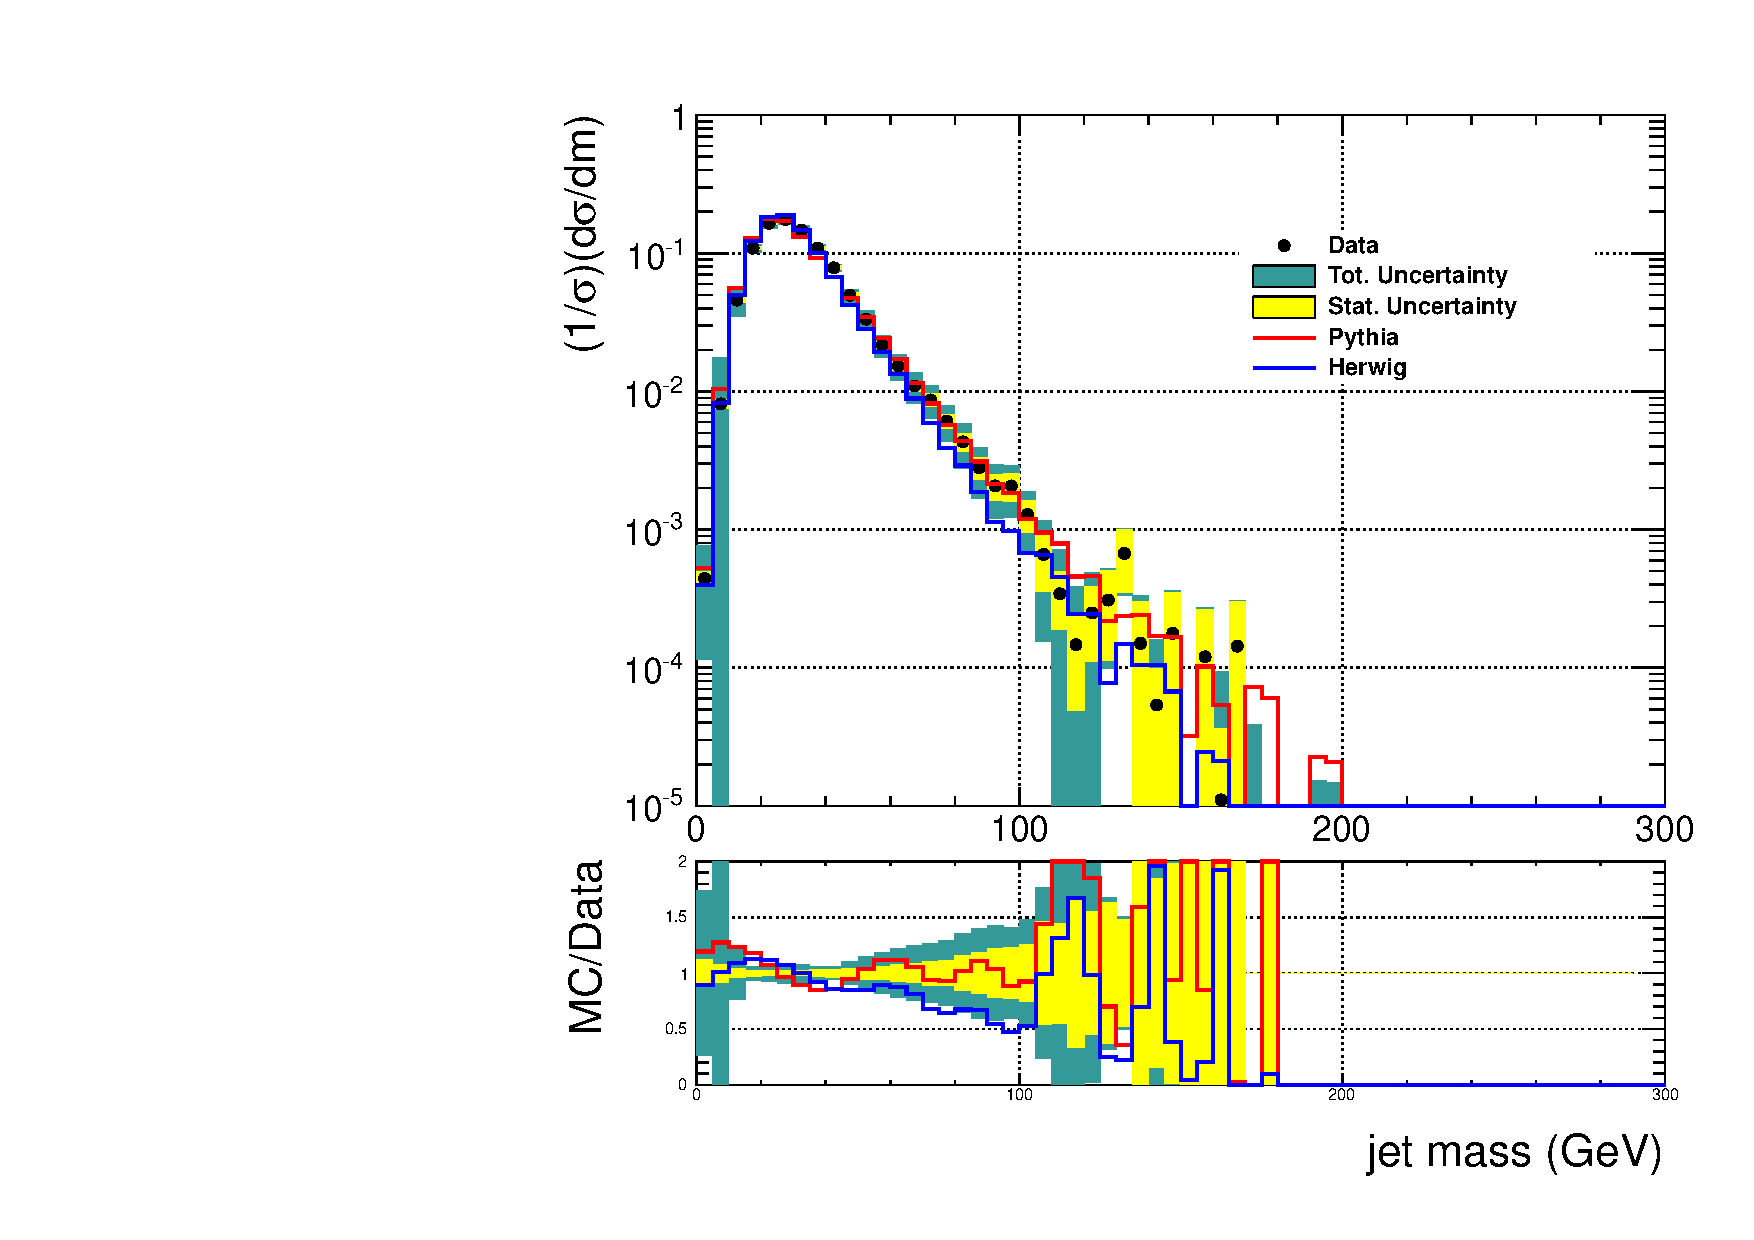
\includegraphics[width=0.49\textwidth]{figs/Zmm/jetmassunf_ak7_allpT.pdf}
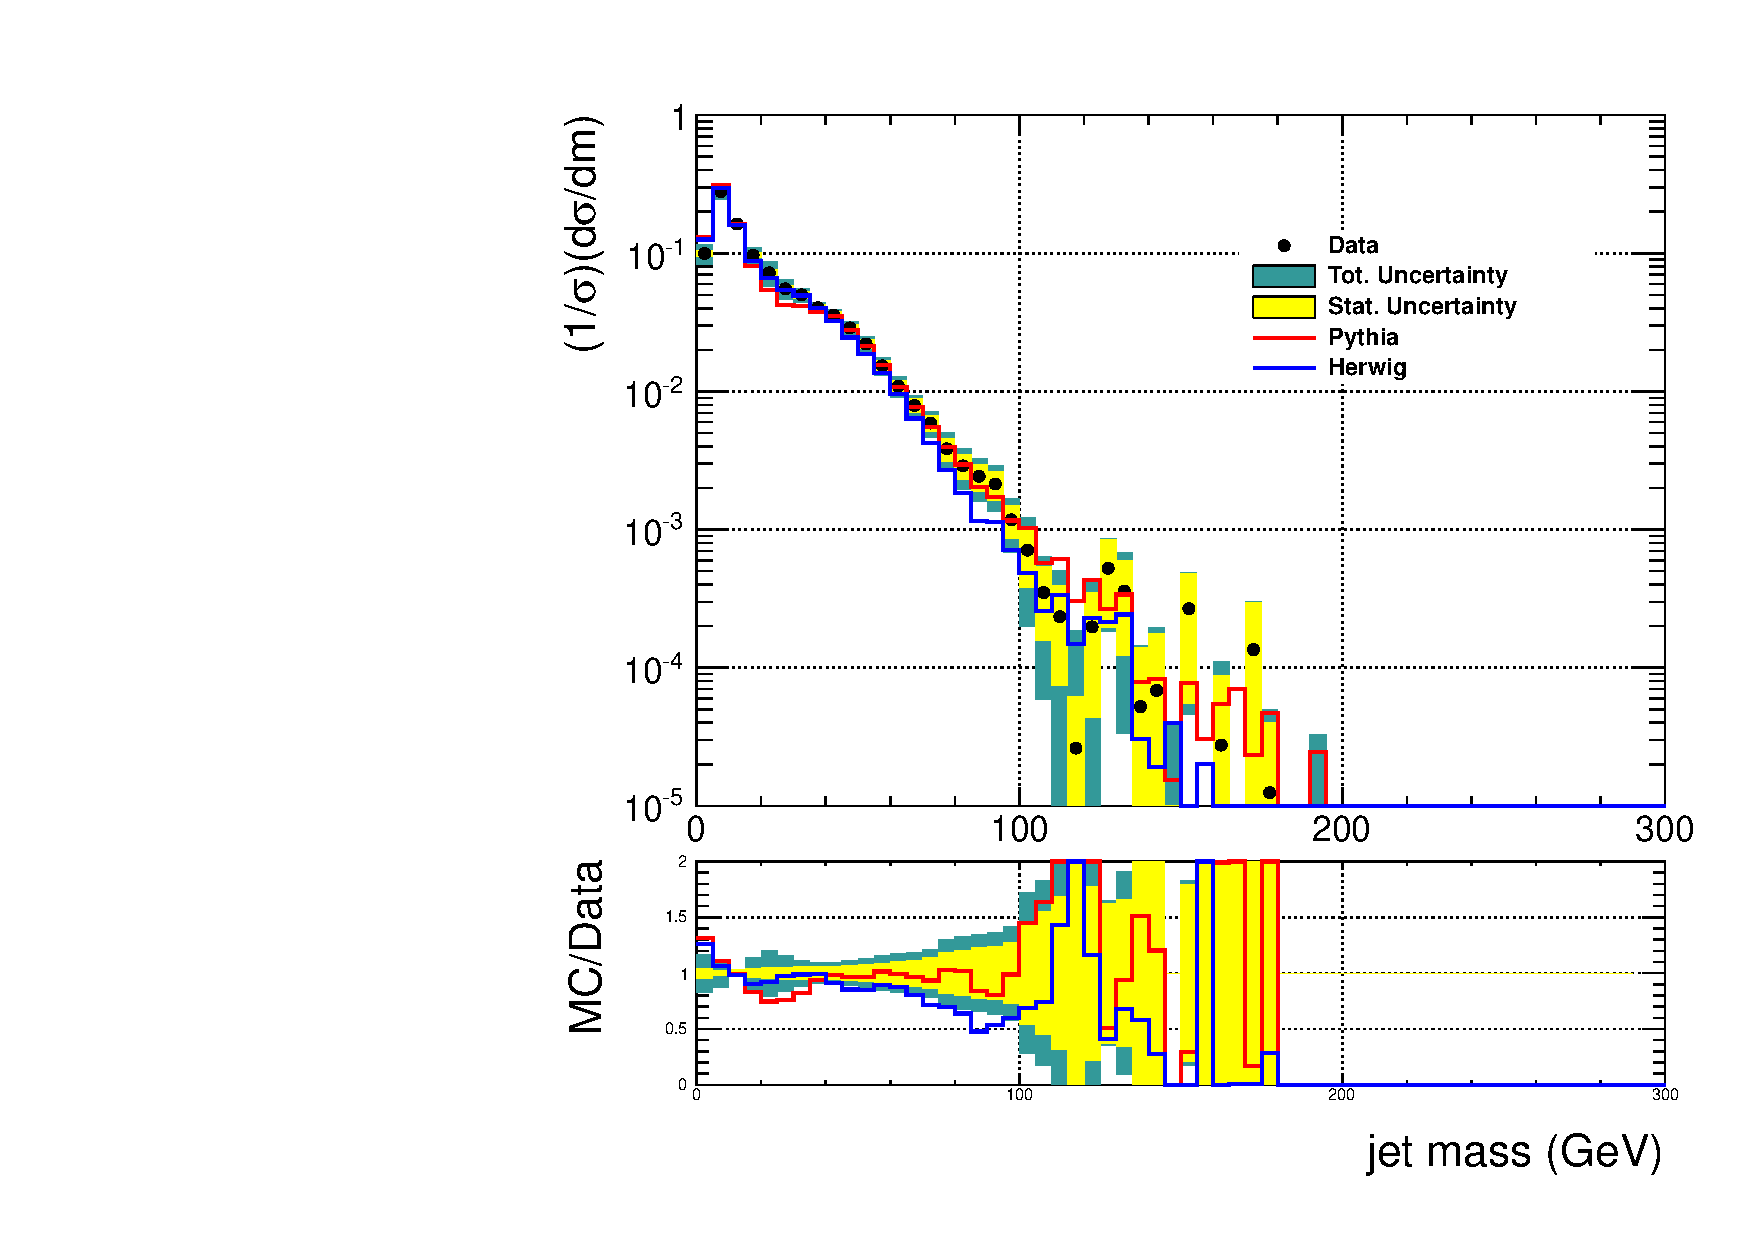
\includegraphics[width=0.49\textwidth]{figs/Zmm/jetmassunf_ak7pr_allpT.pdf}
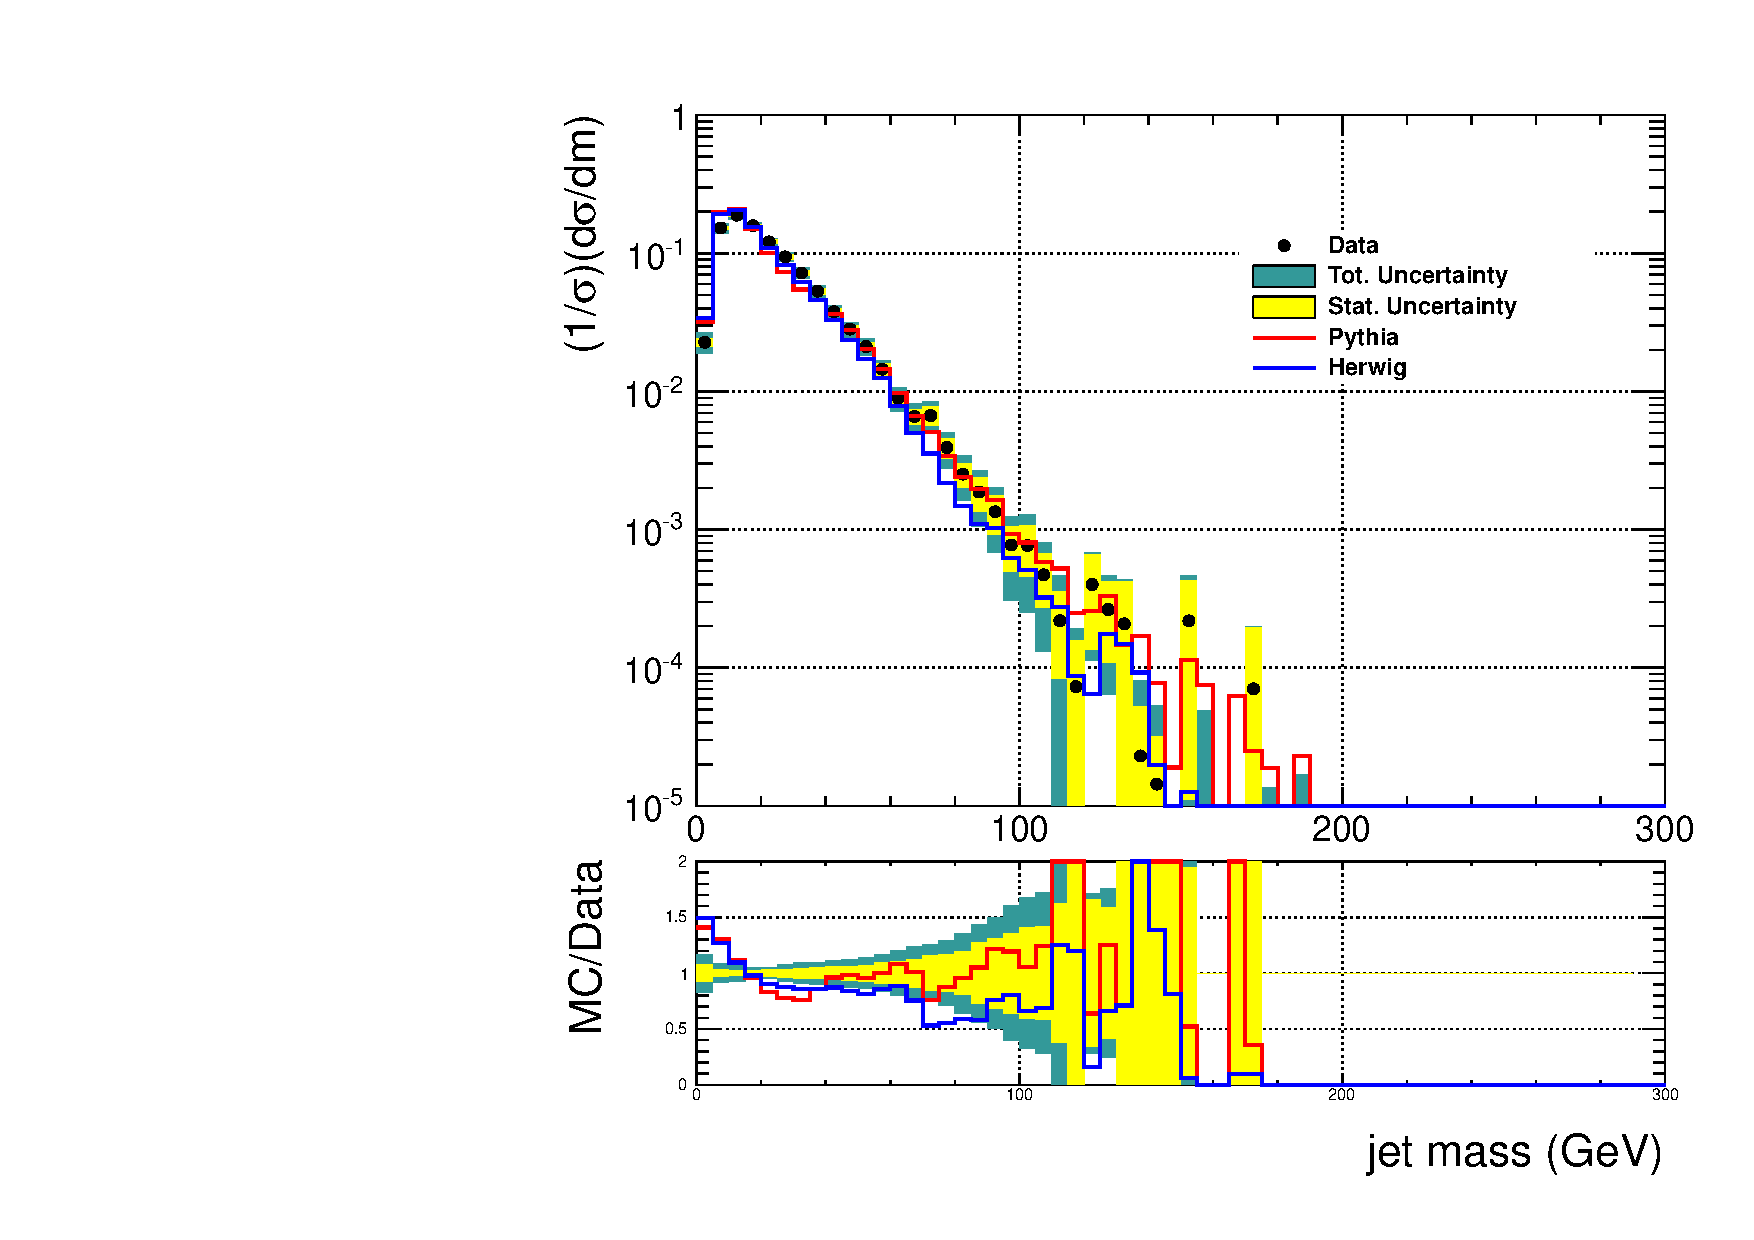
\includegraphics[width=0.49\textwidth]{figs/Zmm/jetmassunf_ak7tr_allpT.pdf}
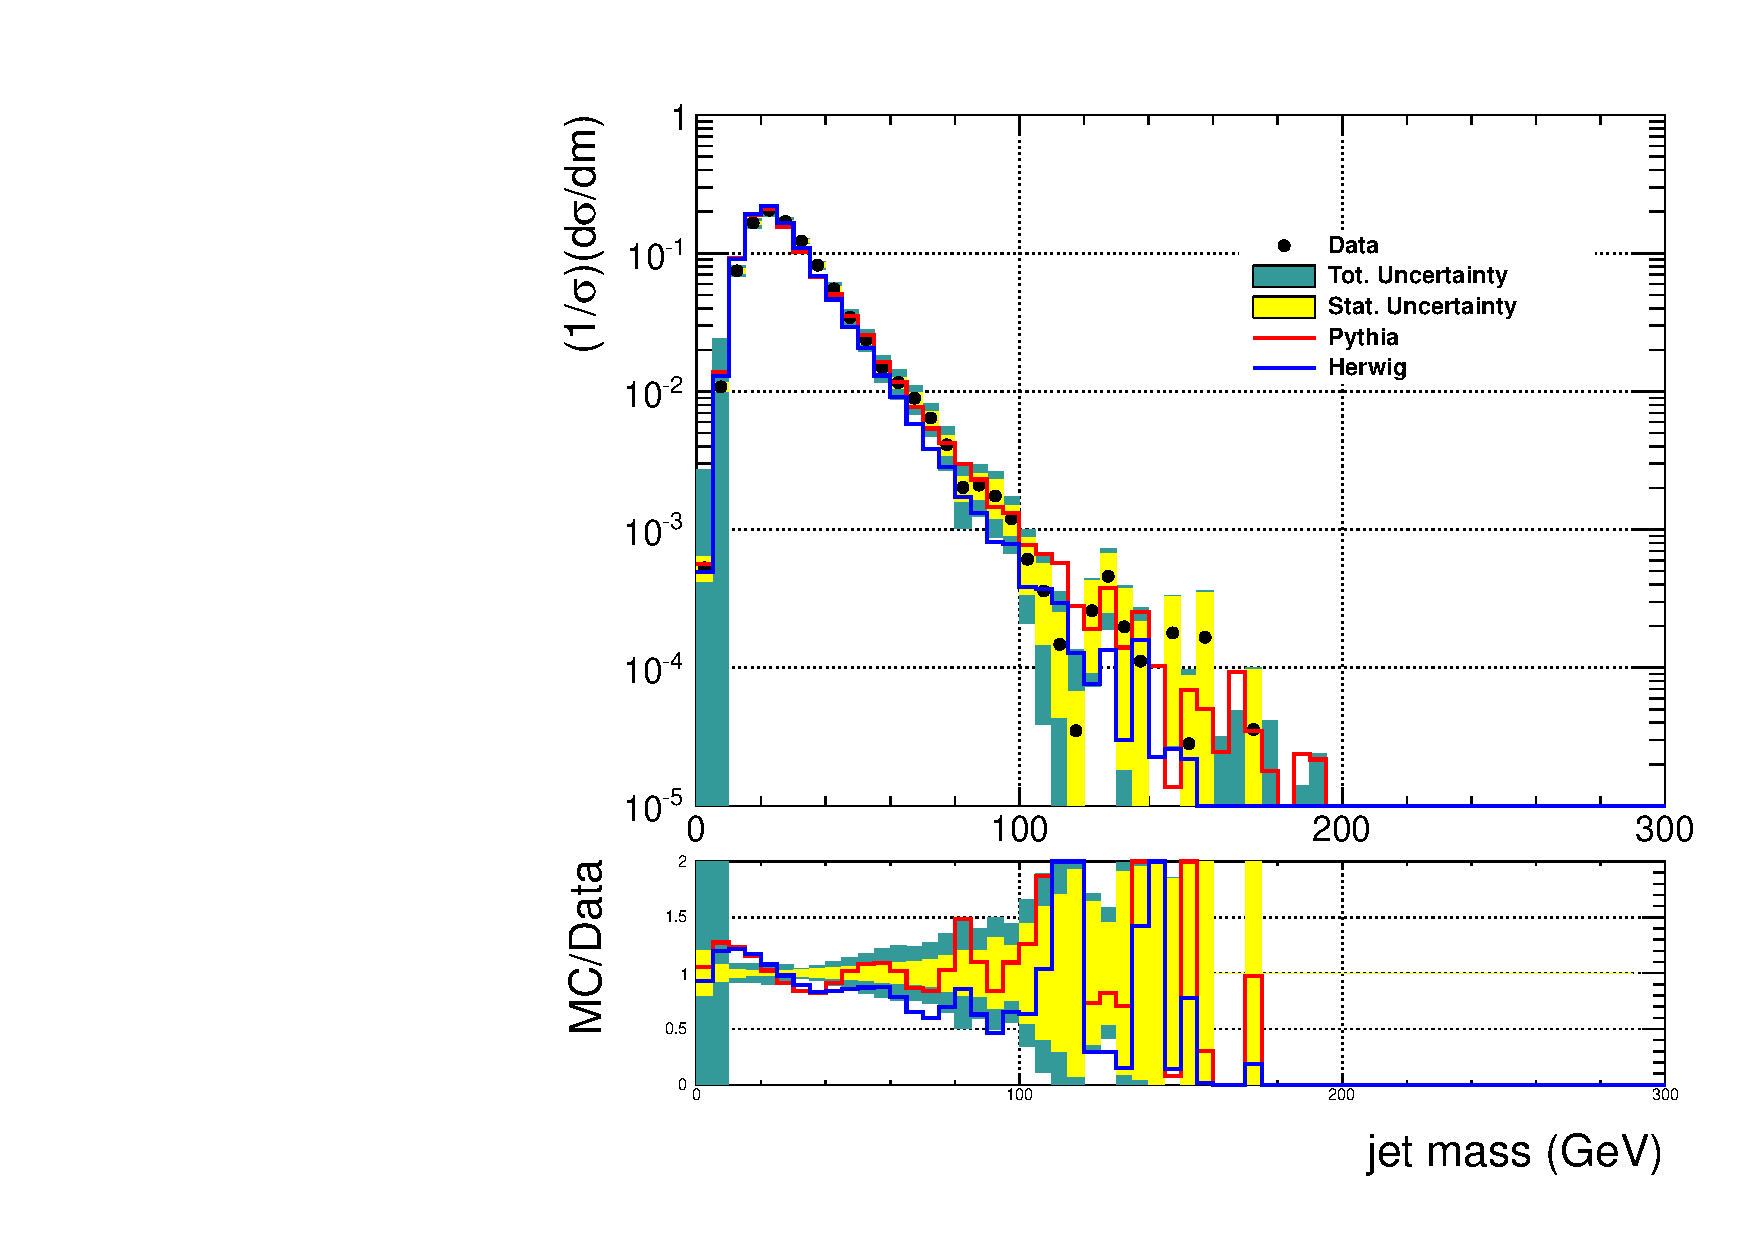
\includegraphics[width=0.49\textwidth]{figs/Zmm/jetmassunf_ak7ft_allpT.pdf}
\caption{Unfolded AK7 ungroomed and groomed jet mass distribution for $Z(\mu\mu)$+ jet events. The data (black points) are compared to the MC expectations from Madgraph (solid red) and herwigpp (solid blue). From the top, in clockwise order: ungroomed, pruned, filtered and trimmed jet mass distributions.}
\label{figs:AK7ZmmInt1}
\end{figure}


Fig.~\ref{figs:prunedZmmInt1} shows the jet mass distribution for pruned CA 0.8 and filtered CA 1.2 jets in Z$(\mu\mu)$ +jet events.
 
\begin{figure}[!htb]
\centering
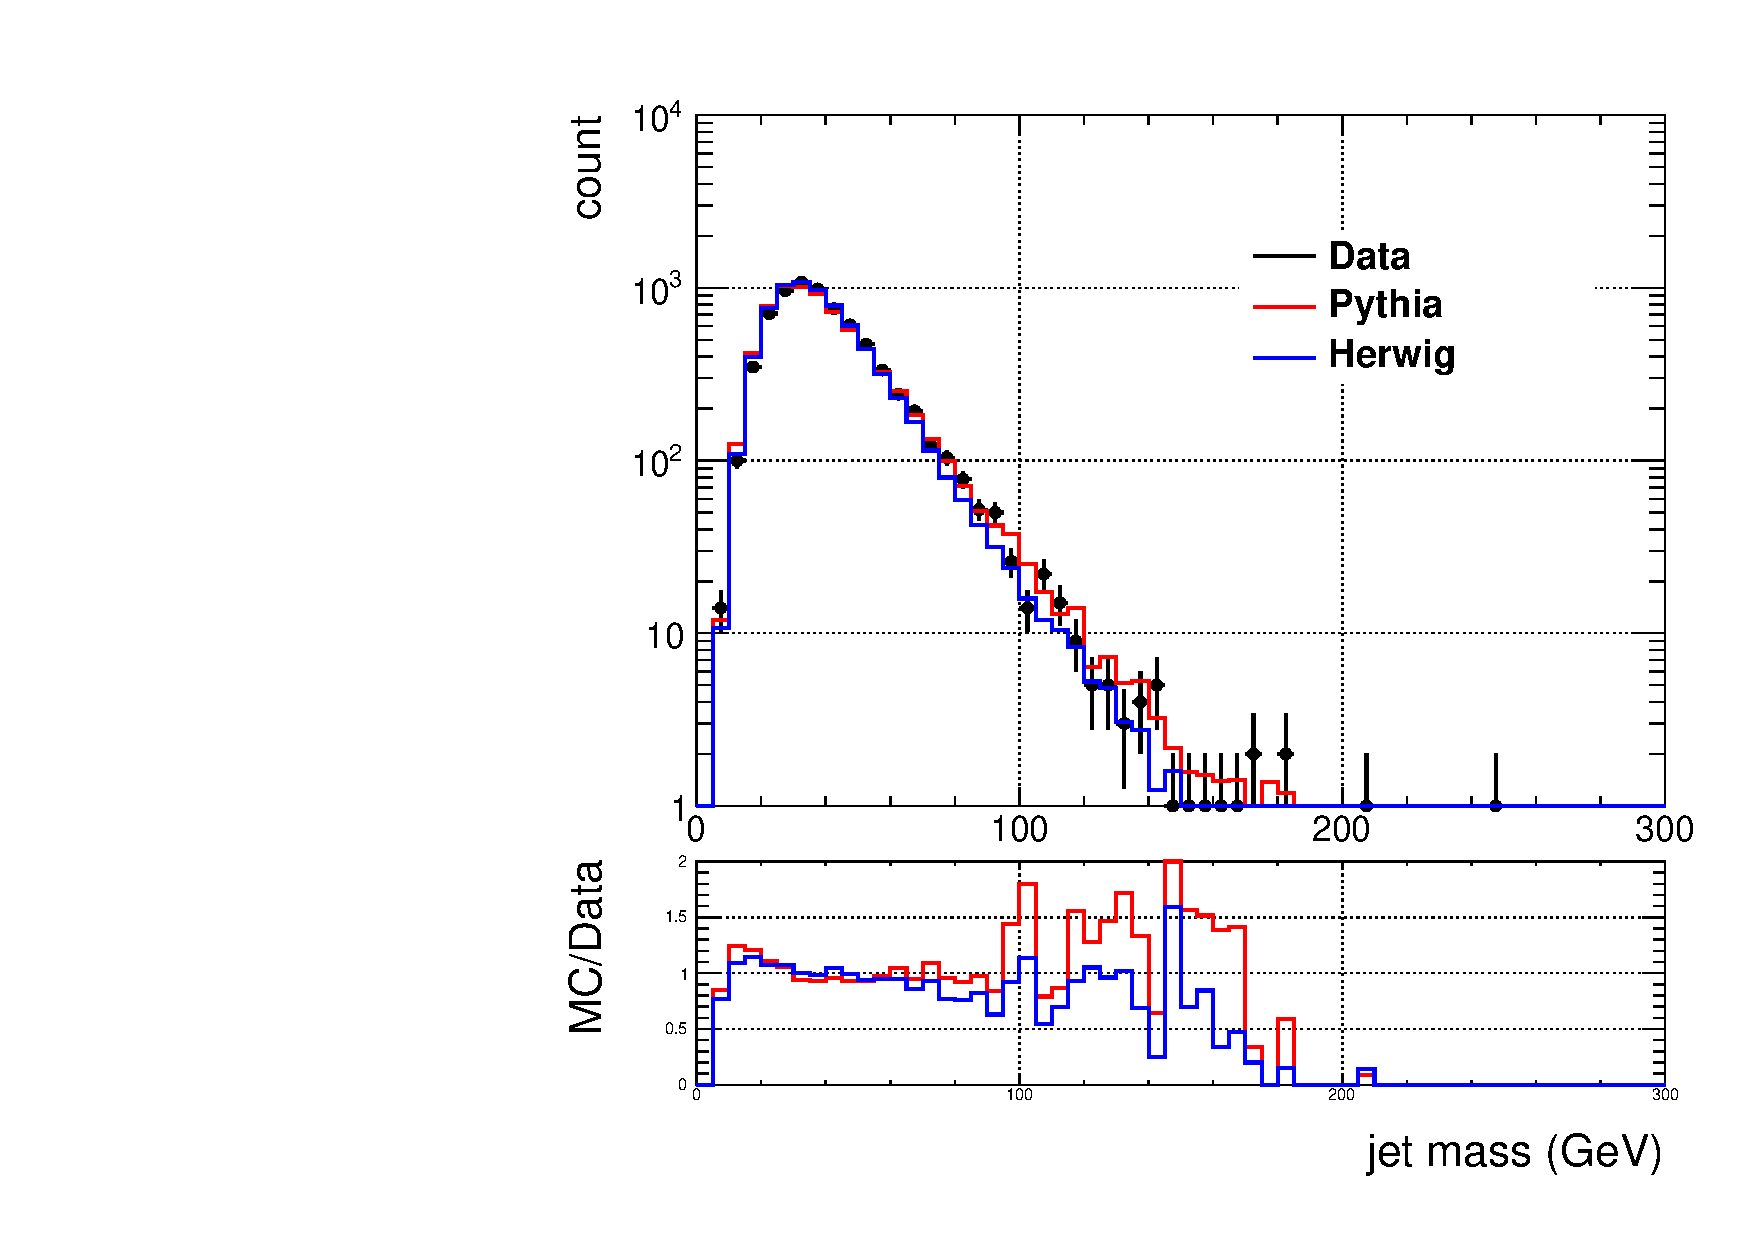
\includegraphics[width=0.49\textwidth]{figs/Zmm/jetmassReco_ca8_allpT.pdf}
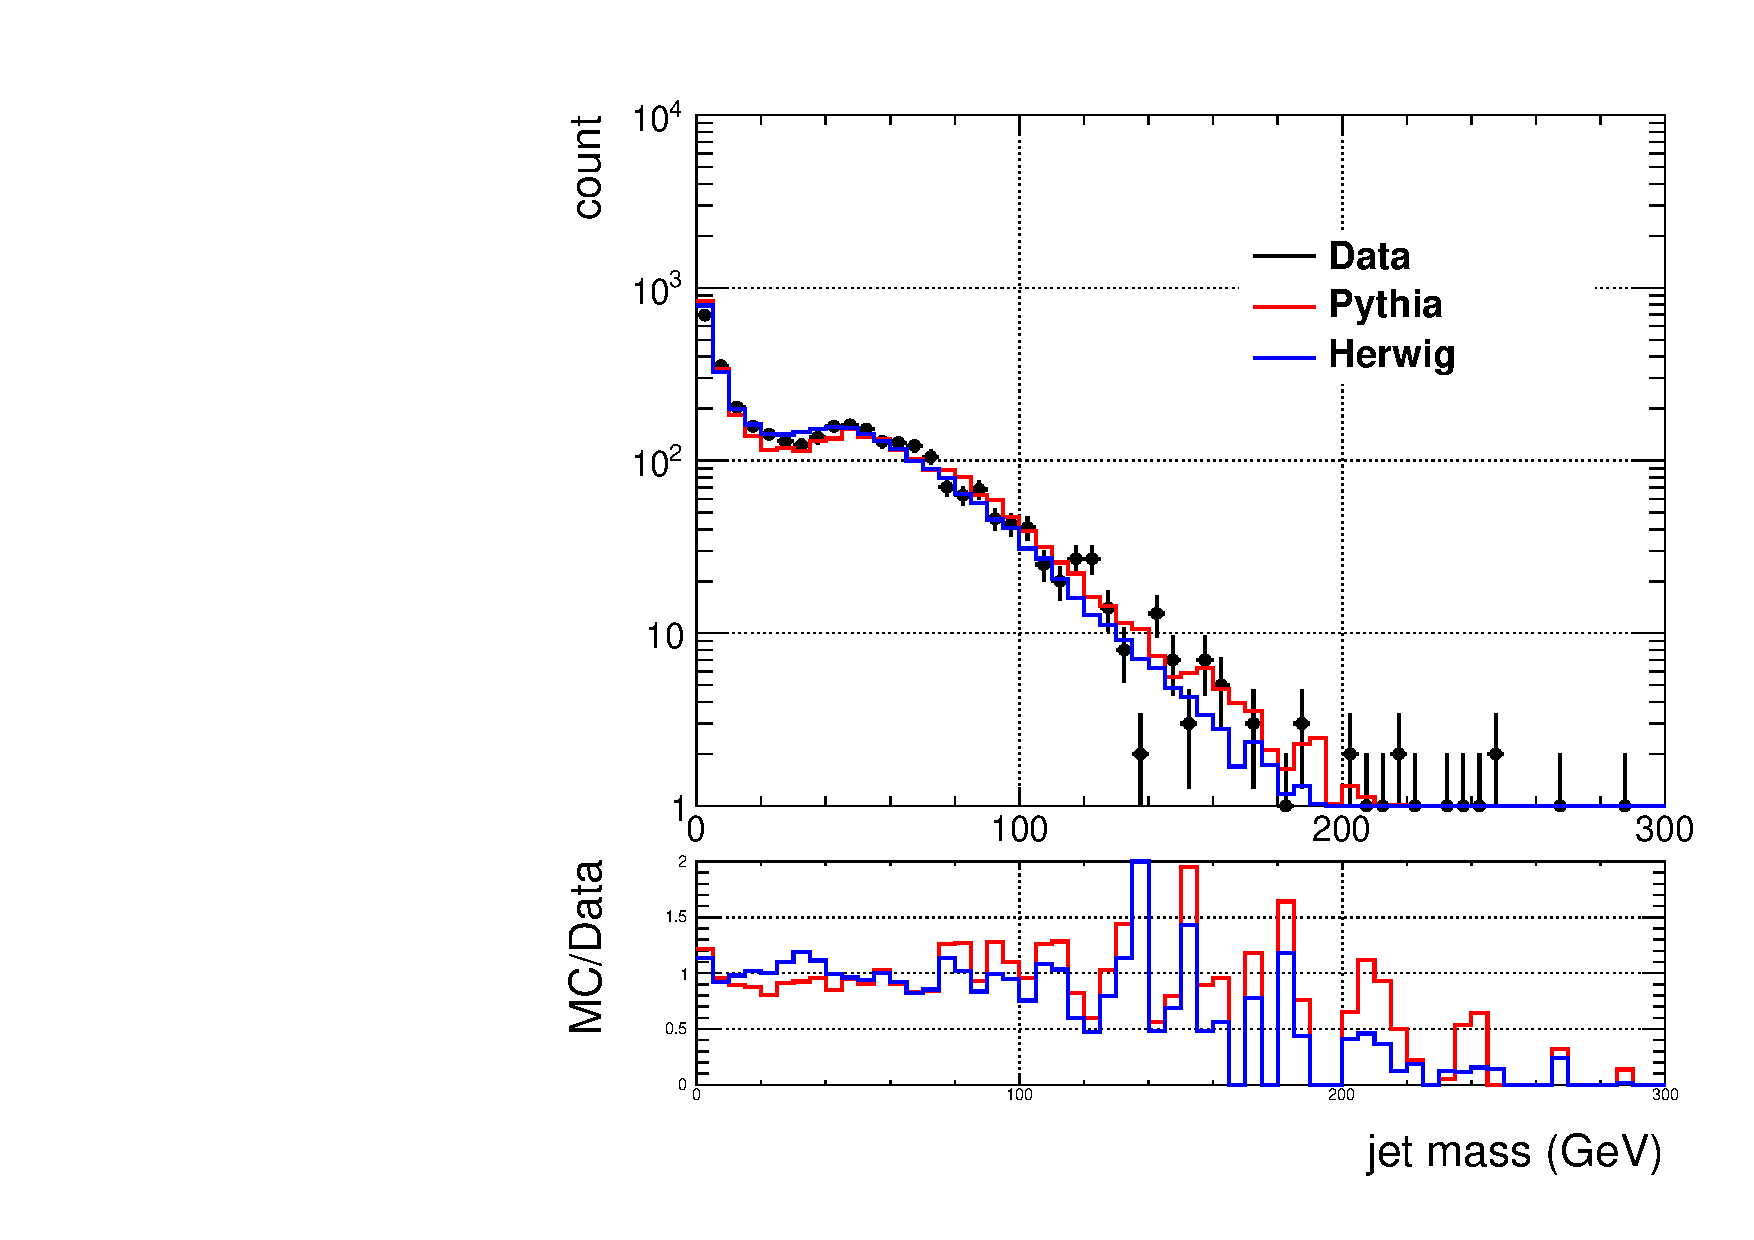
\includegraphics[width=0.49\textwidth]{figs/Zmm/jetmassReco_ca12mdft_allpT.pdf}
\caption{(Not yet Unfolded) CA 0.8 pruned and CA 1.2 filtered jet mass distribution for $Z(\mu\mu)$+ jet events. The data (black points) are compared to the MC expectations from Madgraph (solid red) and herwigpp (solid blue).}
\label{figs:prunedZmmInt1}
\end{figure}

\clearpage

\subsection{$Z(ee)$ + jet Analysis}

Fig.~\ref{figs:AK7ZeeInt1} shows the jet mass distribution for AK7 jets in Z$(ee)$ +jet events, for the different clustering algorithm studied: ungroomed, pruned, trimmed and filtered respectively.

\begin{figure}[!htb]
\centering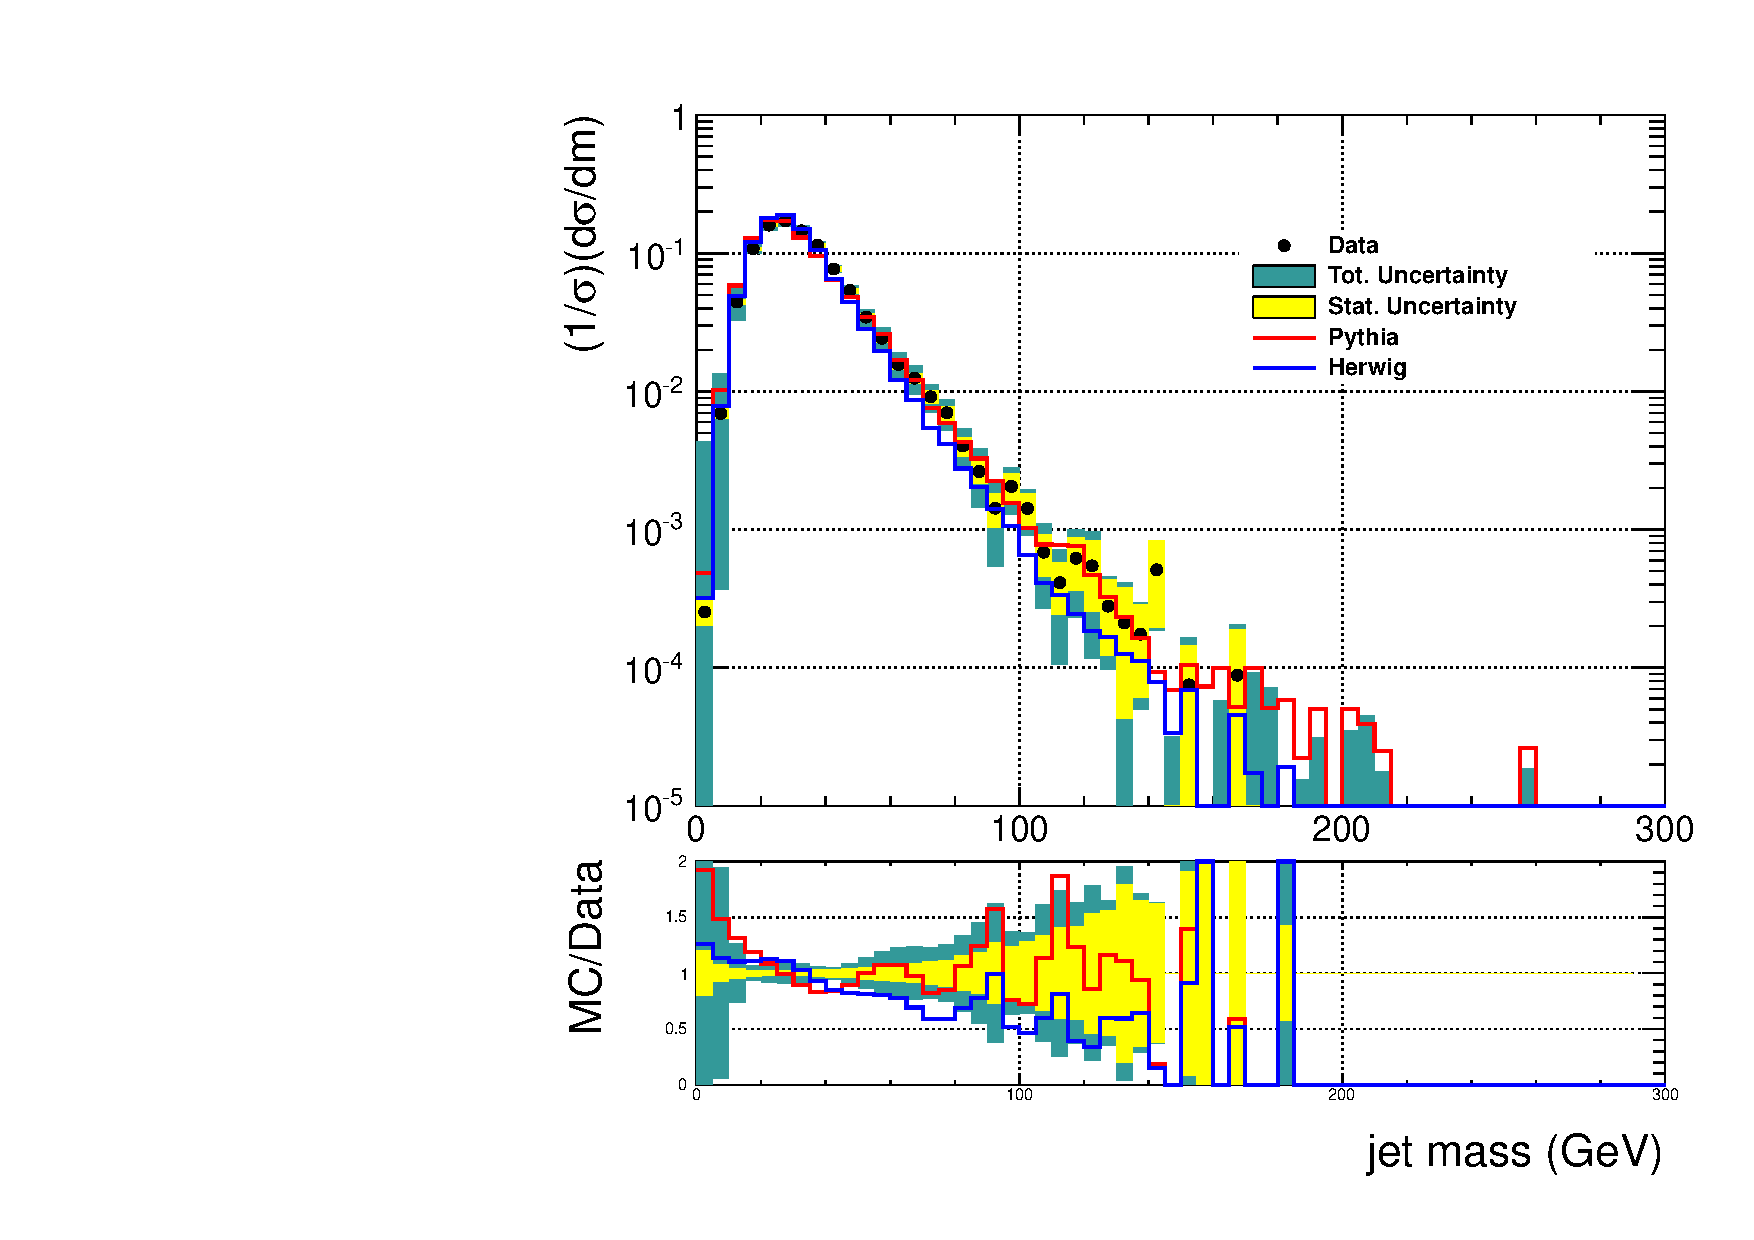
\includegraphics[width=0.49\textwidth]{figs/Zee/jetmassunf_ak7_allpT.pdf}
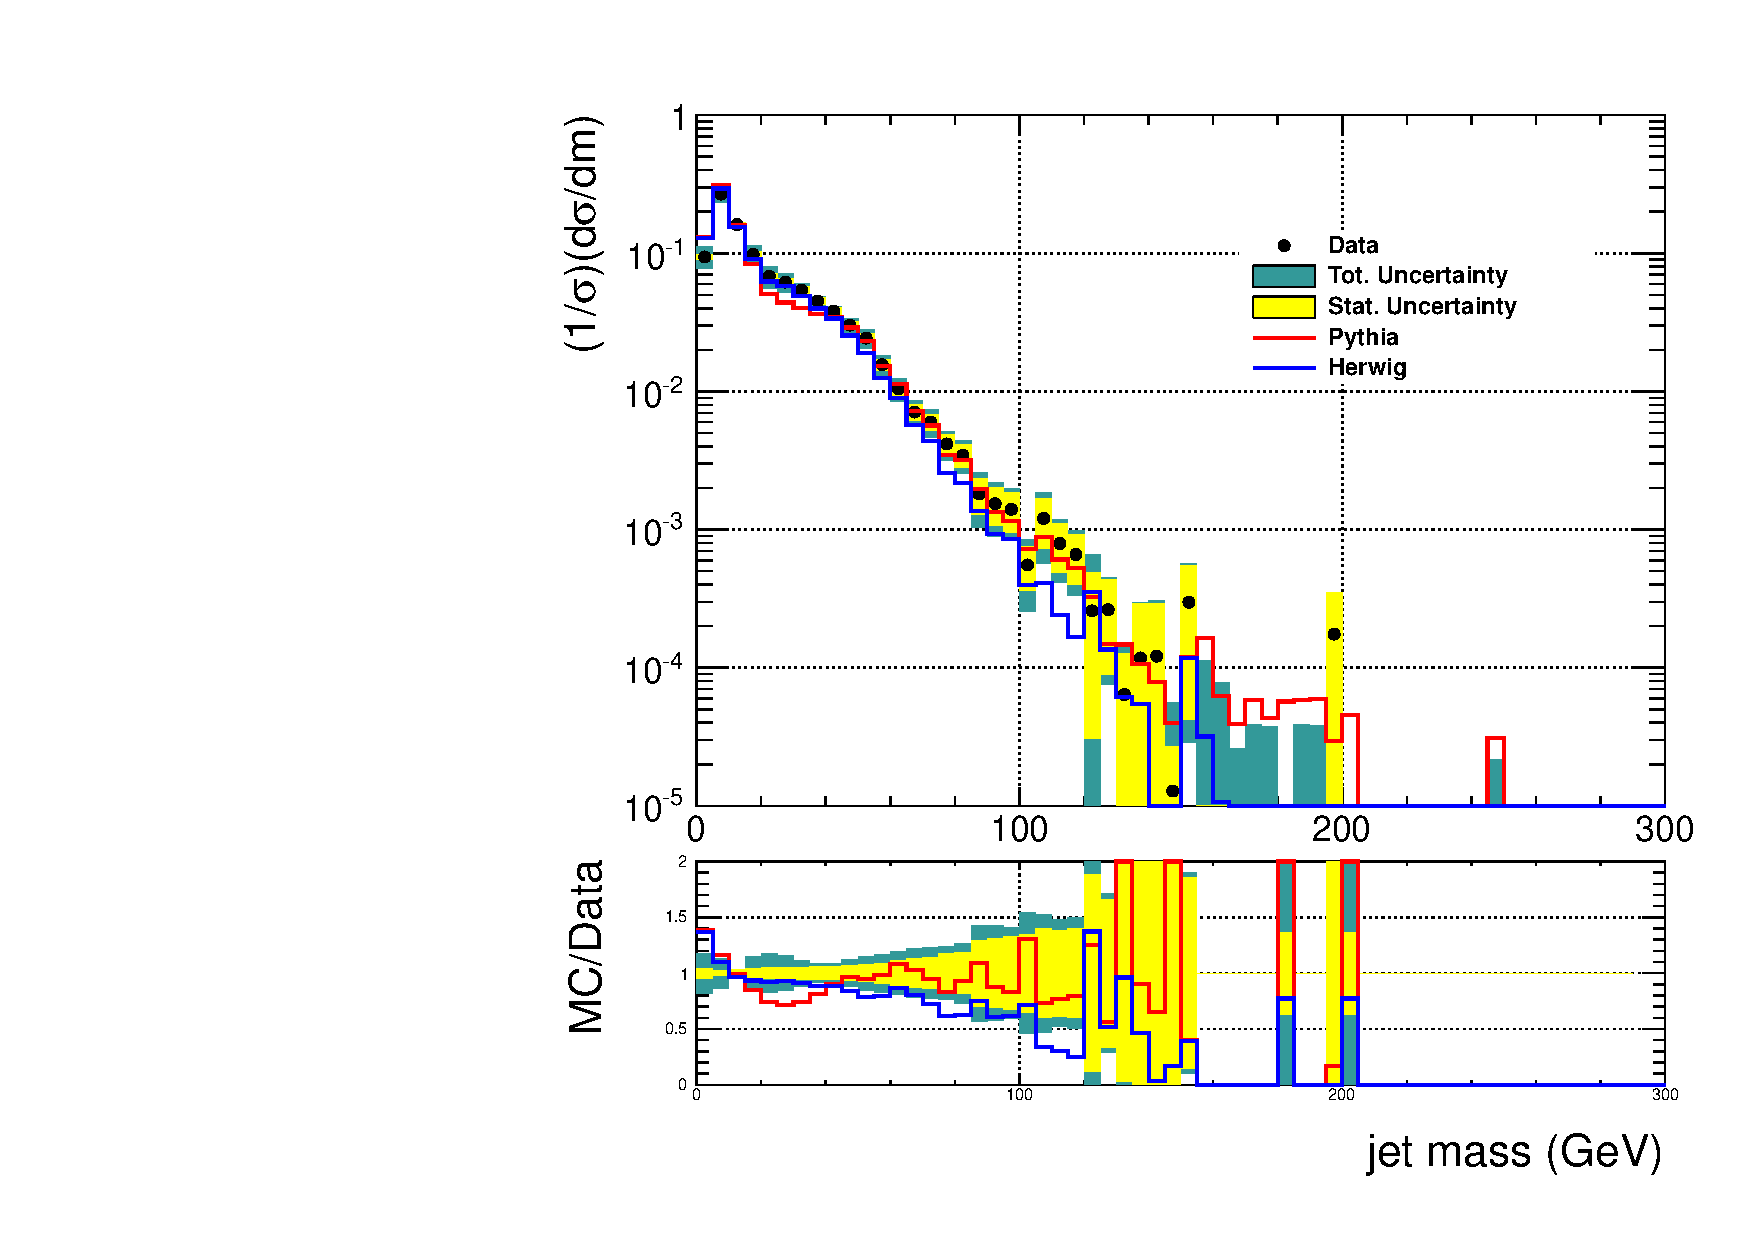
\includegraphics[width=0.49\textwidth]{figs/Zee/jetmassunf_ak7pr_allpT.pdf}
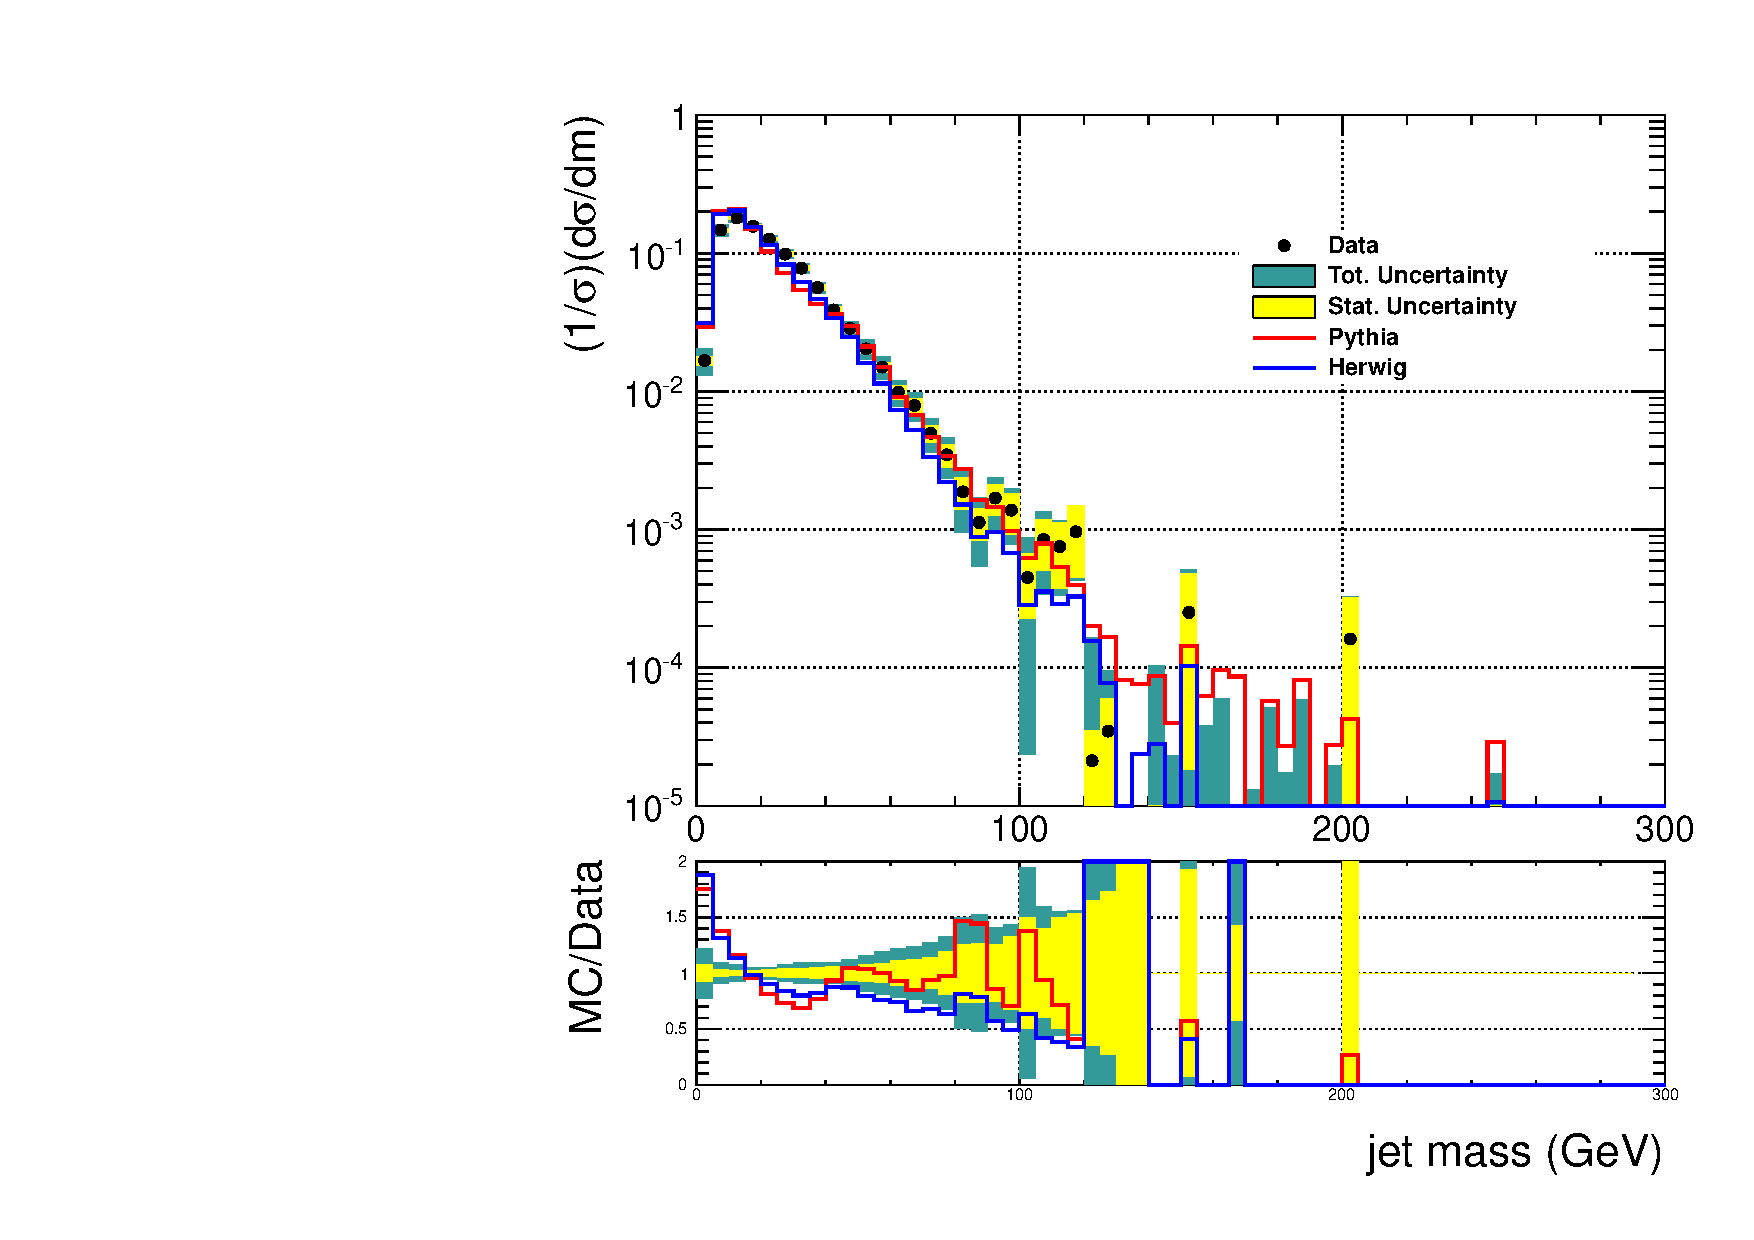
\includegraphics[width=0.49\textwidth]{figs/Zee/jetmassunf_ak7tr_allpT.pdf}
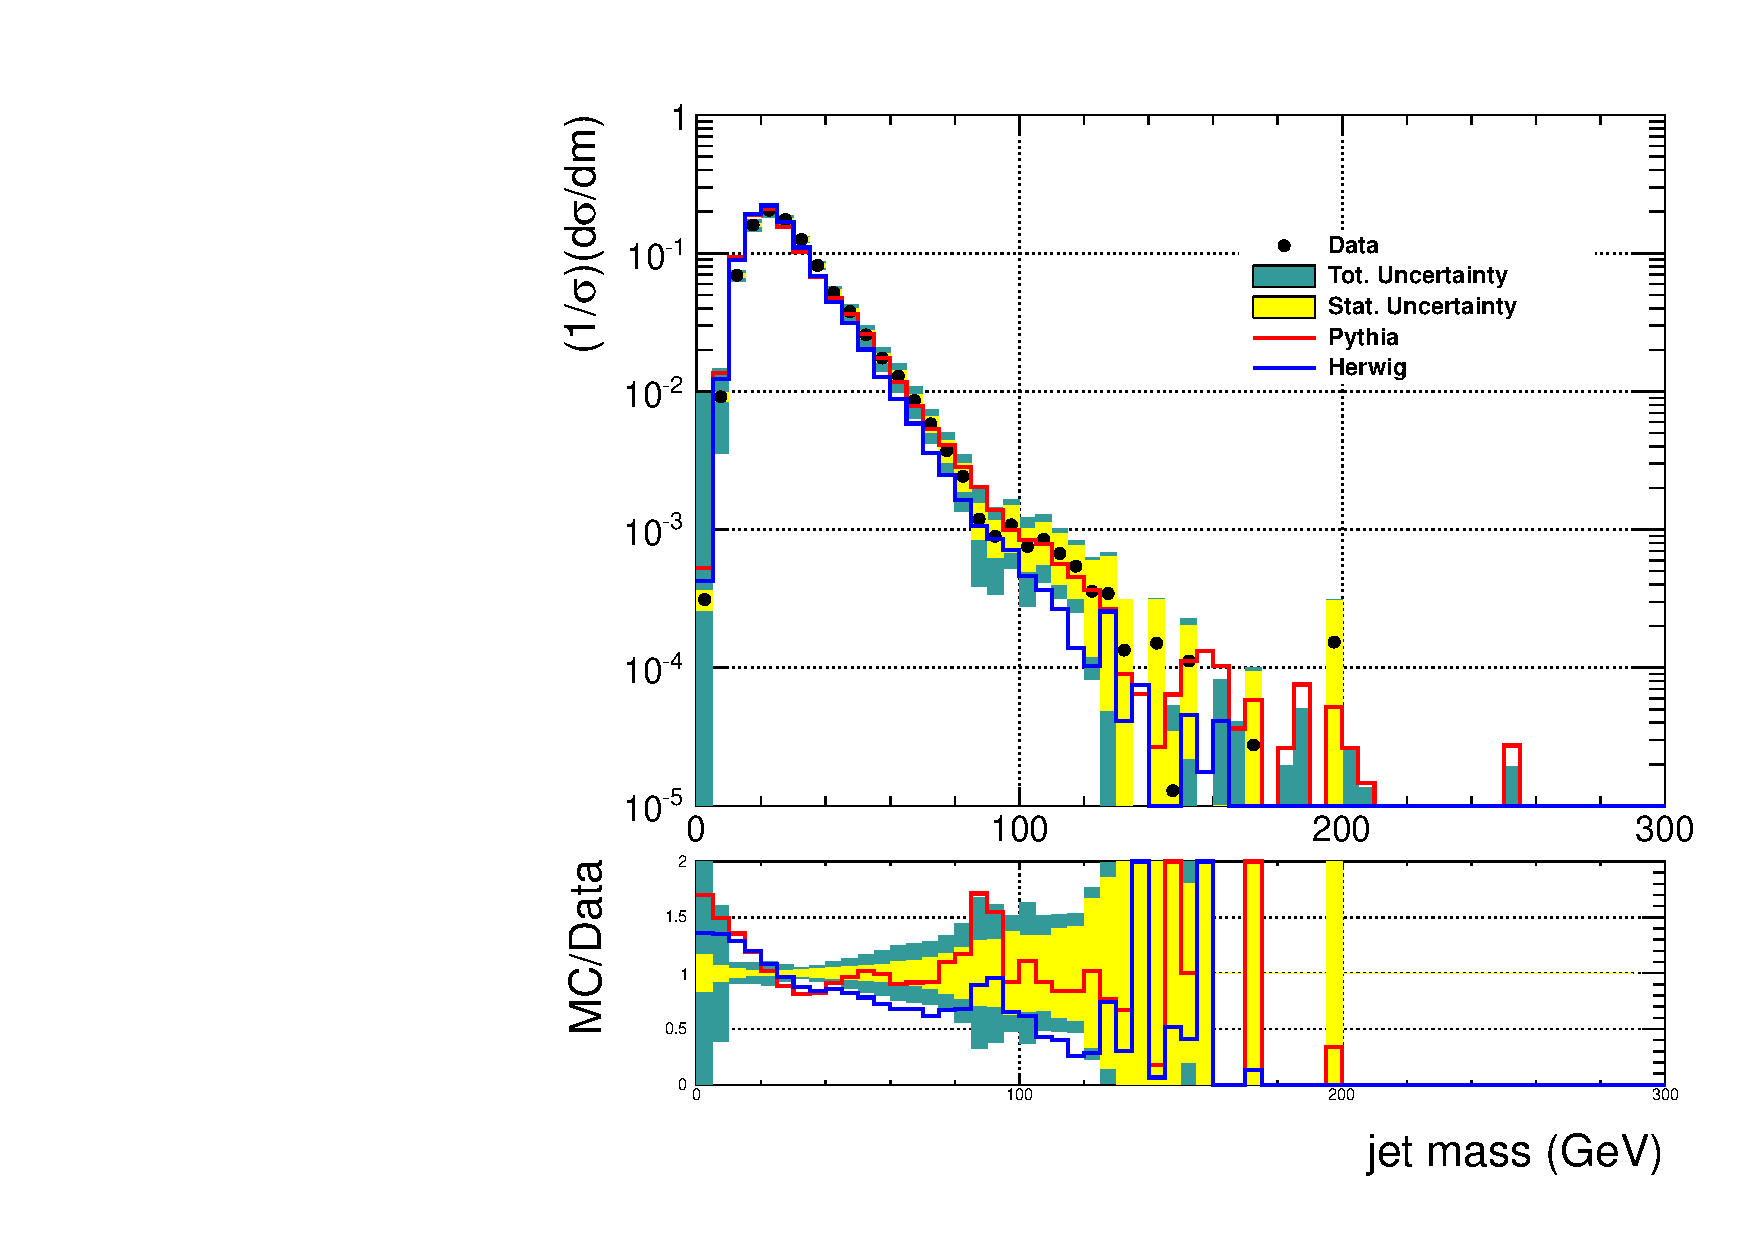
\includegraphics[width=0.49\textwidth]{figs/Zee/jetmassunf_ak7ft_allpT.pdf}
\caption{Unfolded AK7 ungroomed and groomed jet mass distribution for $Z(ee)$+ jet events. The data (black points) are compared to the MC expectations from Madgraph (solid red) and herwigpp (solid blue). From the top, in clockwise order: ungroomed, pruned, filtered and trimmed jet mass distributions.}
\label{figs:AK7ZeeInt1}
\end{figure}



Fig.~\ref{figs:prunedZeeInt1} shows the jet mass distribution for pruned CA 0.8 and filtered CA 1.2 jets in Z$(ee)$ +jet events.

\begin{figure}[!htb]
\centering
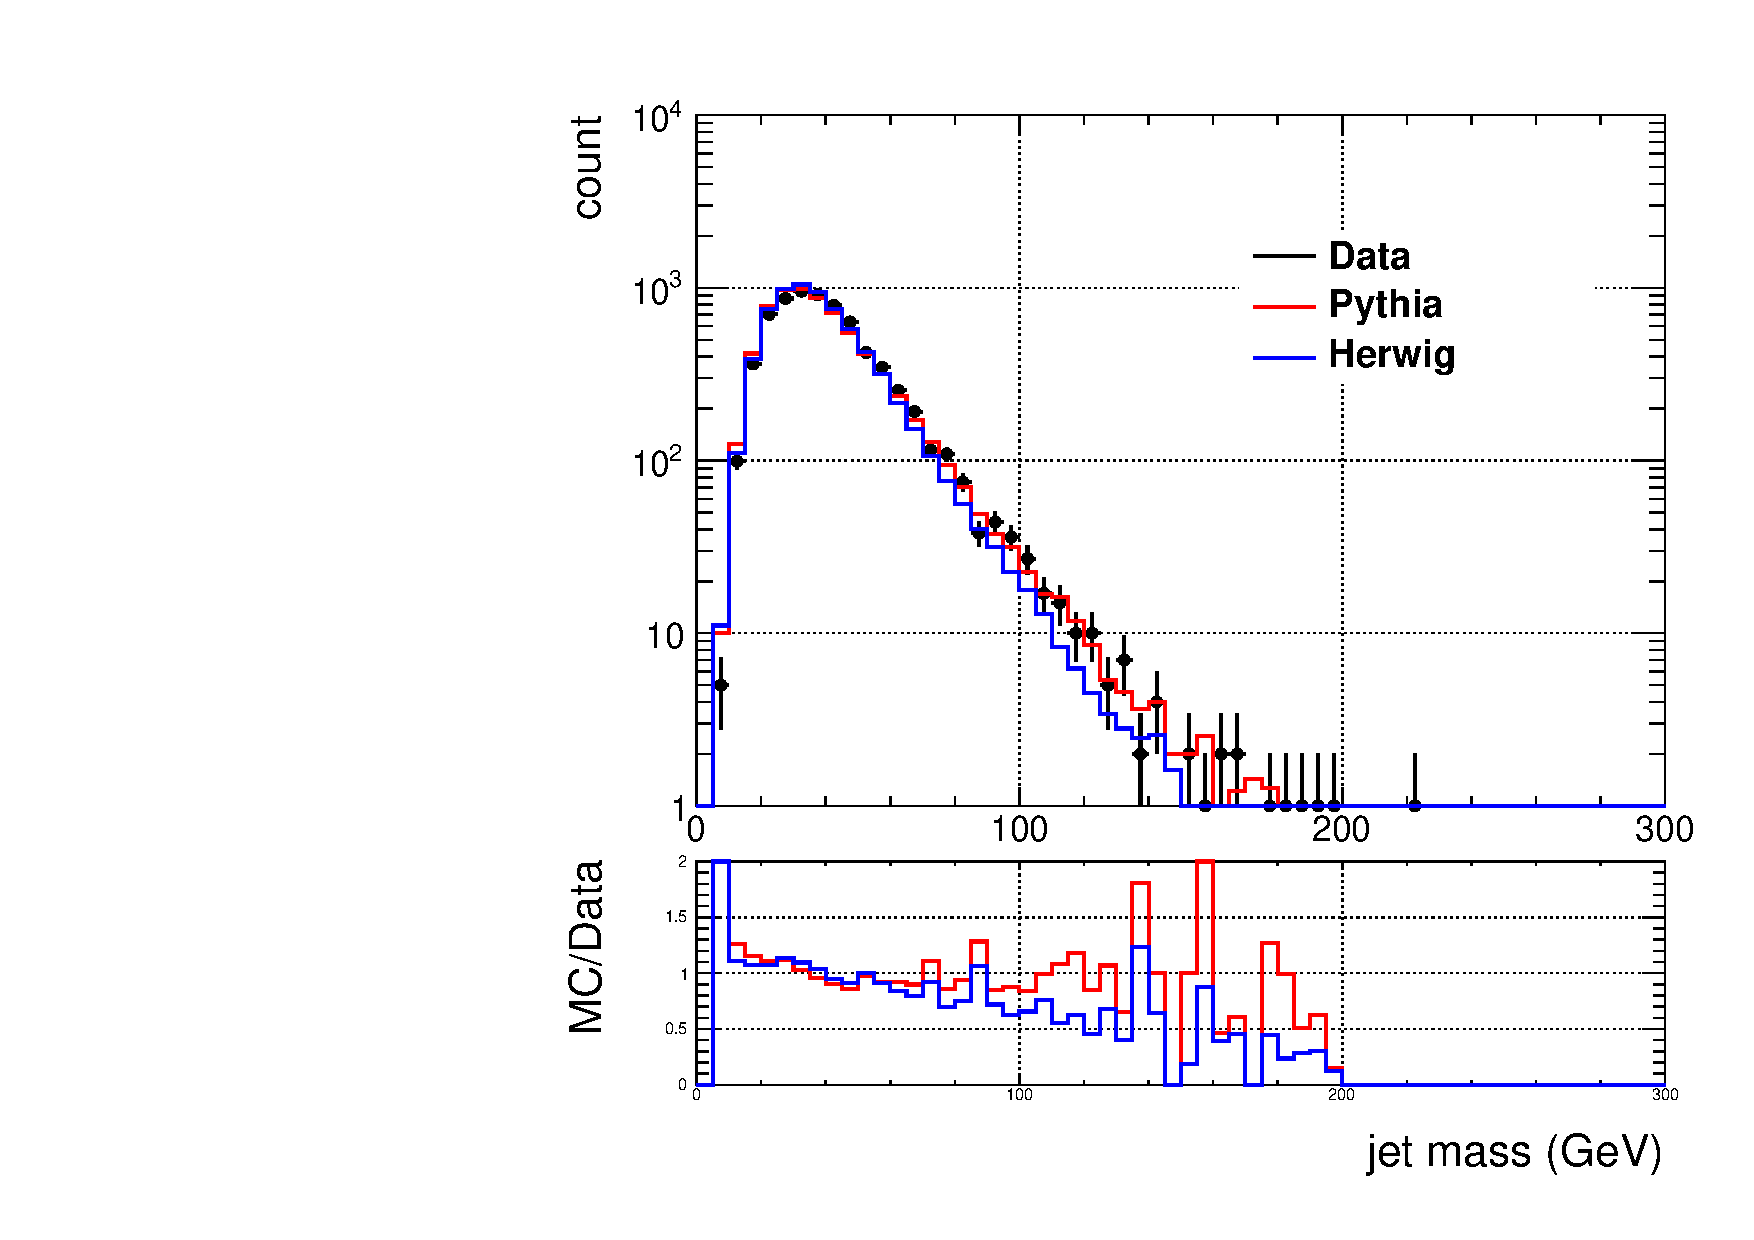
\includegraphics[width=0.49\textwidth]{figs/Zee/jetmassReco_ca8_allpT.pdf}
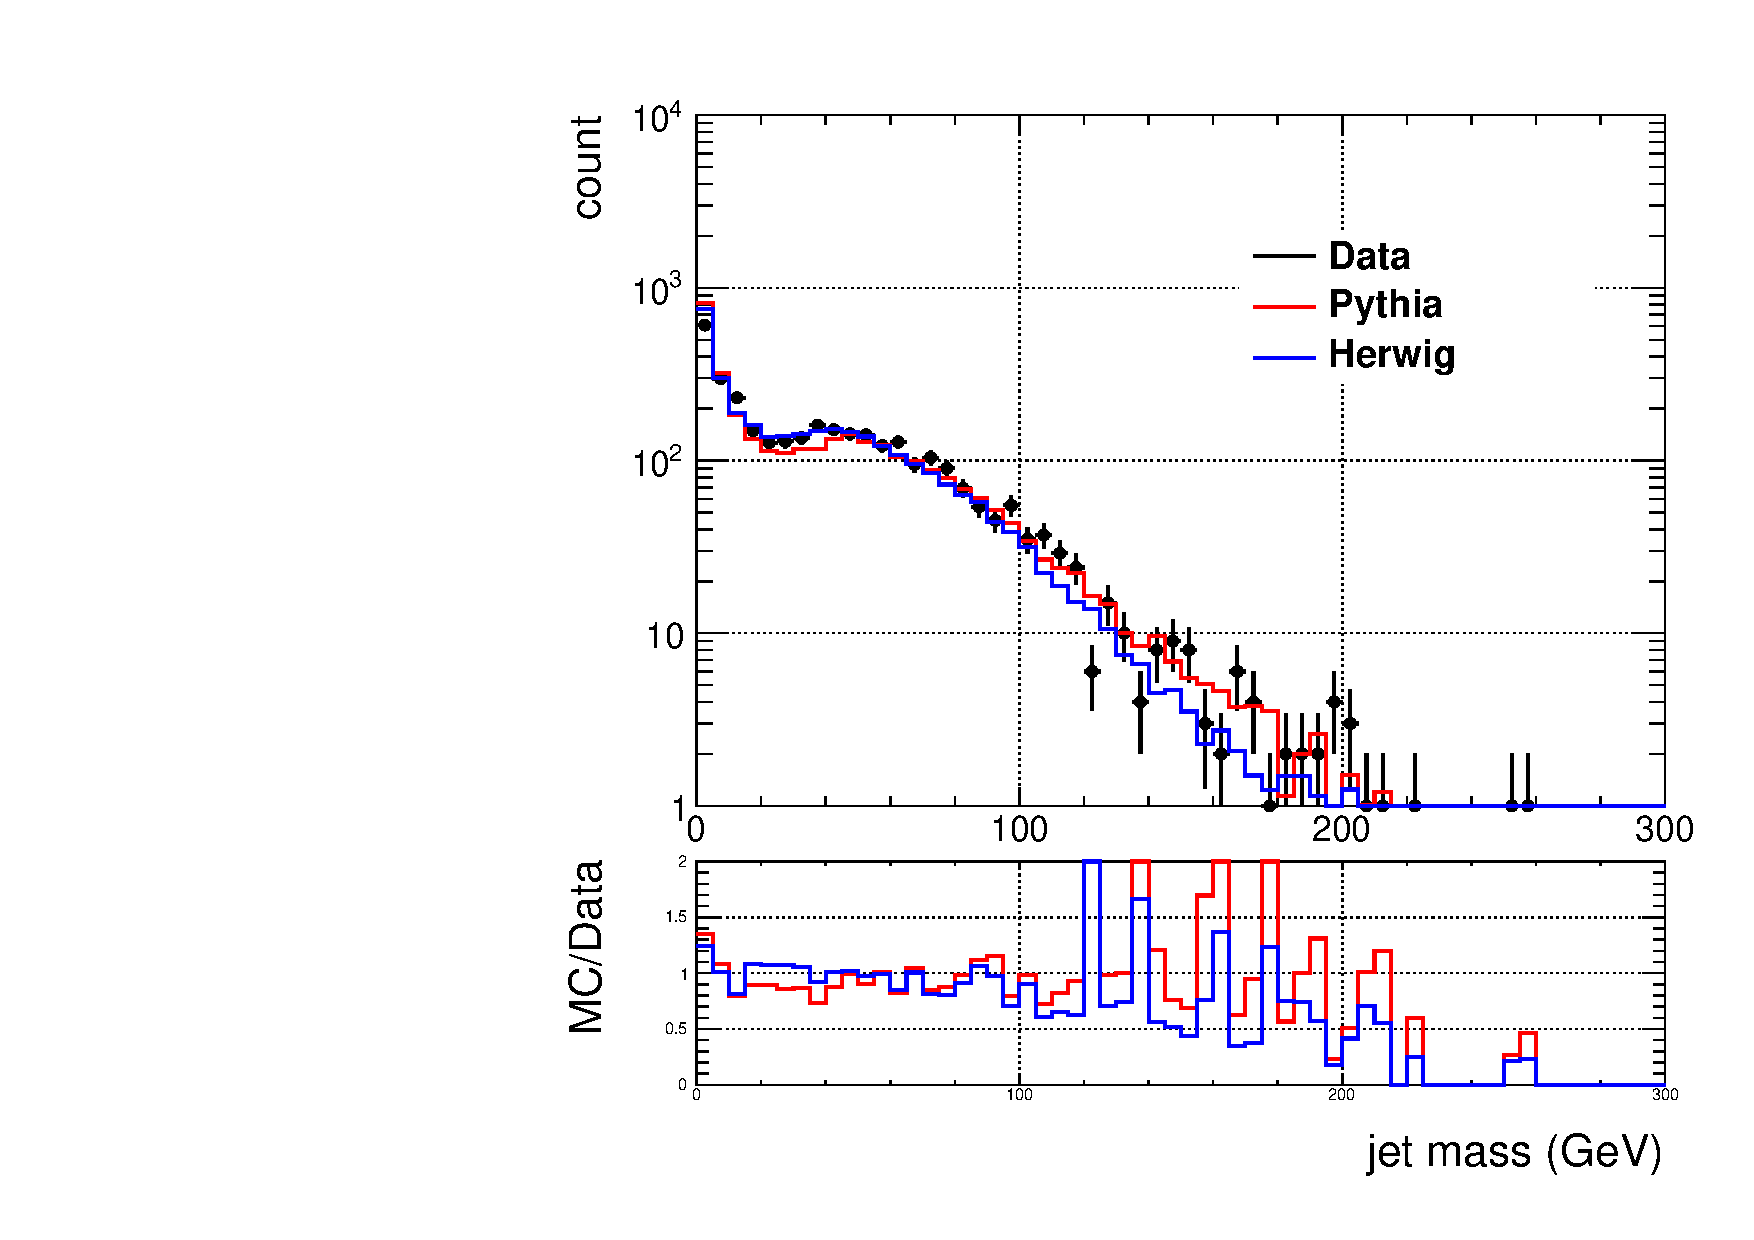
\includegraphics[width=0.49\textwidth]{figs/Zee/jetmassReco_ca12mdft_allpT.pdf}
\caption{(Not yet Unfolded) CA 0.8 pruned and CA 1.2 filtered jet mass distribution for $Z(ee)$+ jet events. The data (black points) are compared to the MC expectations from Madgraph (solid red) and herwigpp (solid blue).}
\label{figs:prunedZeeInt1}
\end{figure}

\clearpage


\subsection{$W(\mu\nu)$ + jet Analysis}

Fig.~\ref{figs:AK7WmnInt1} shows the jet mass distribution for AK7 jets in W$(\mu\nu)$ +jet events, for the different clustering algorithm studied: ungroomed, pruned, trimmed and filtered respectively.

\begin{figure}[!htb]\centering
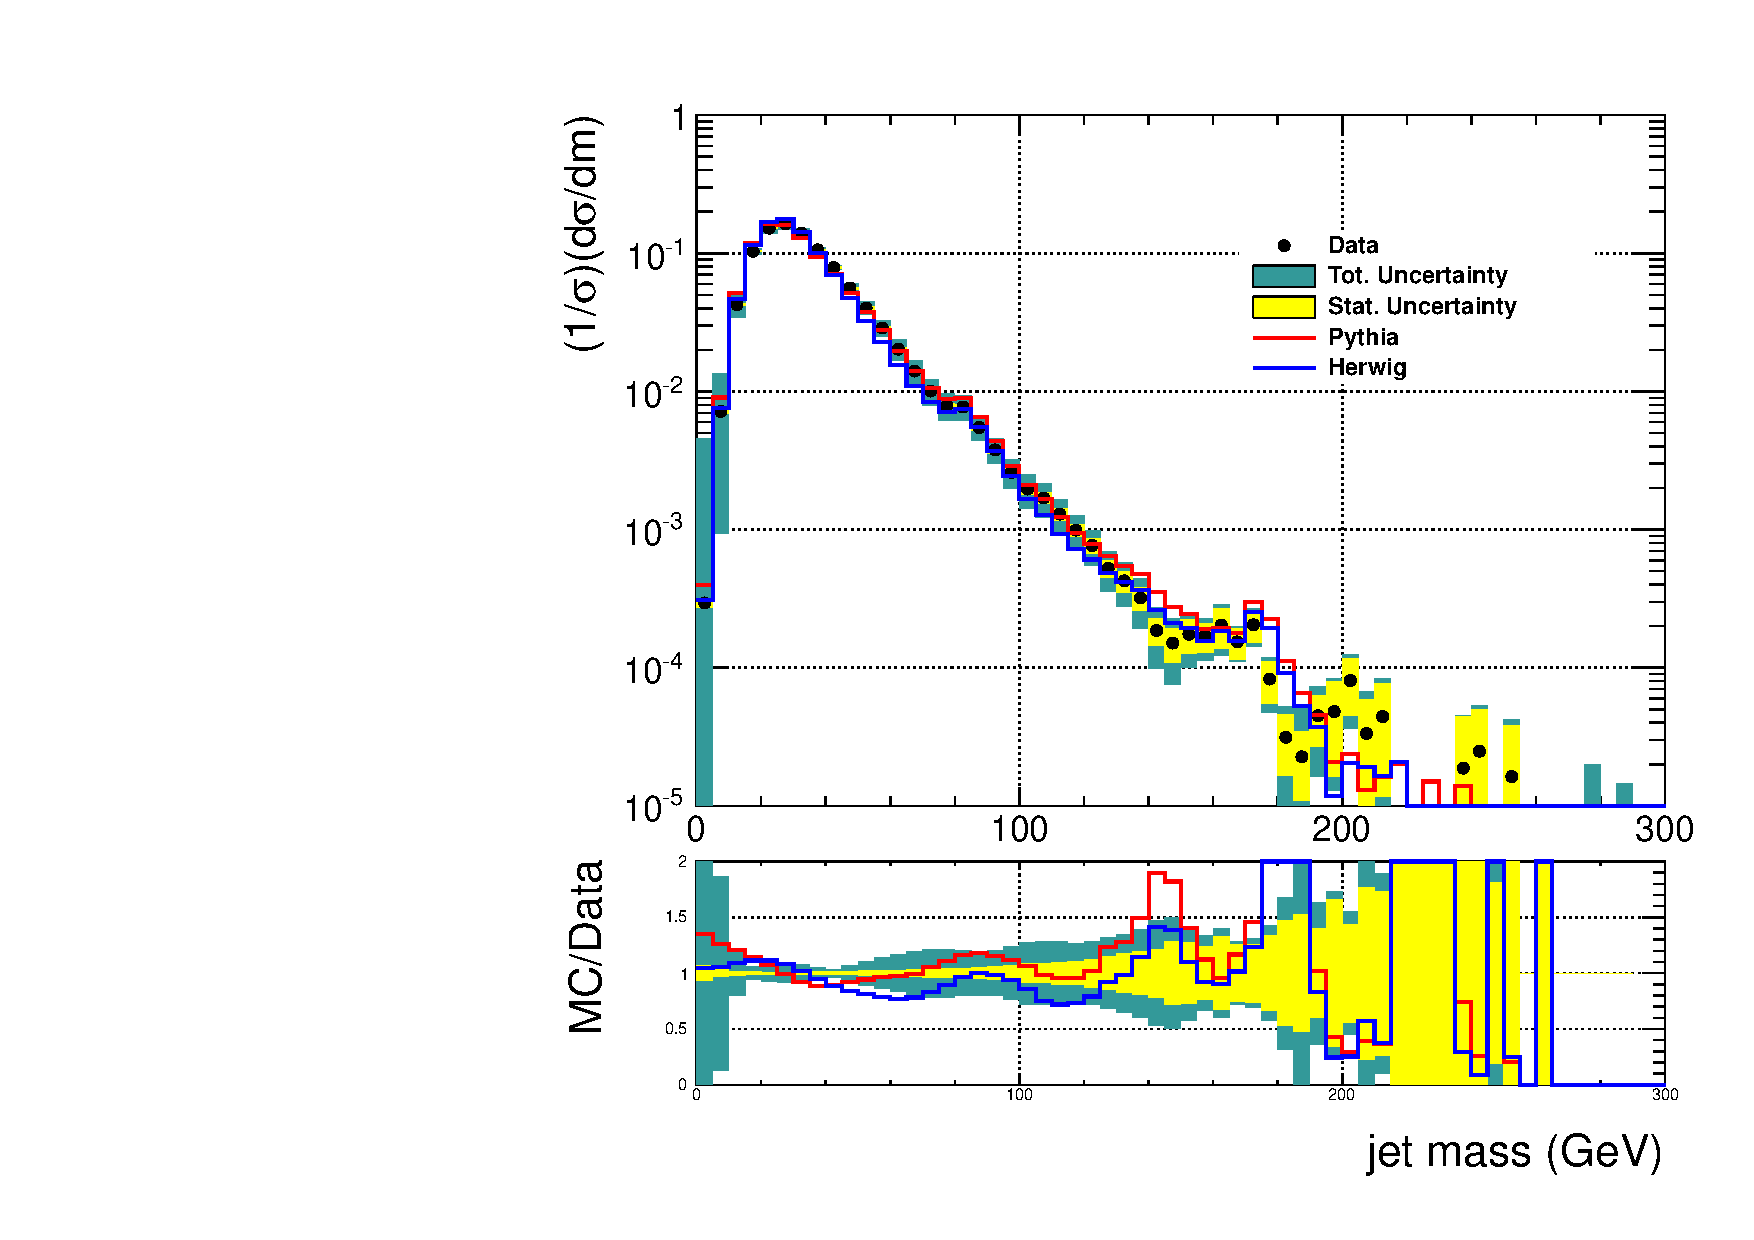
\includegraphics[width=0.49\textwidth]{figs/Wmn/jetmassunf_ak7_allpT.pdf}
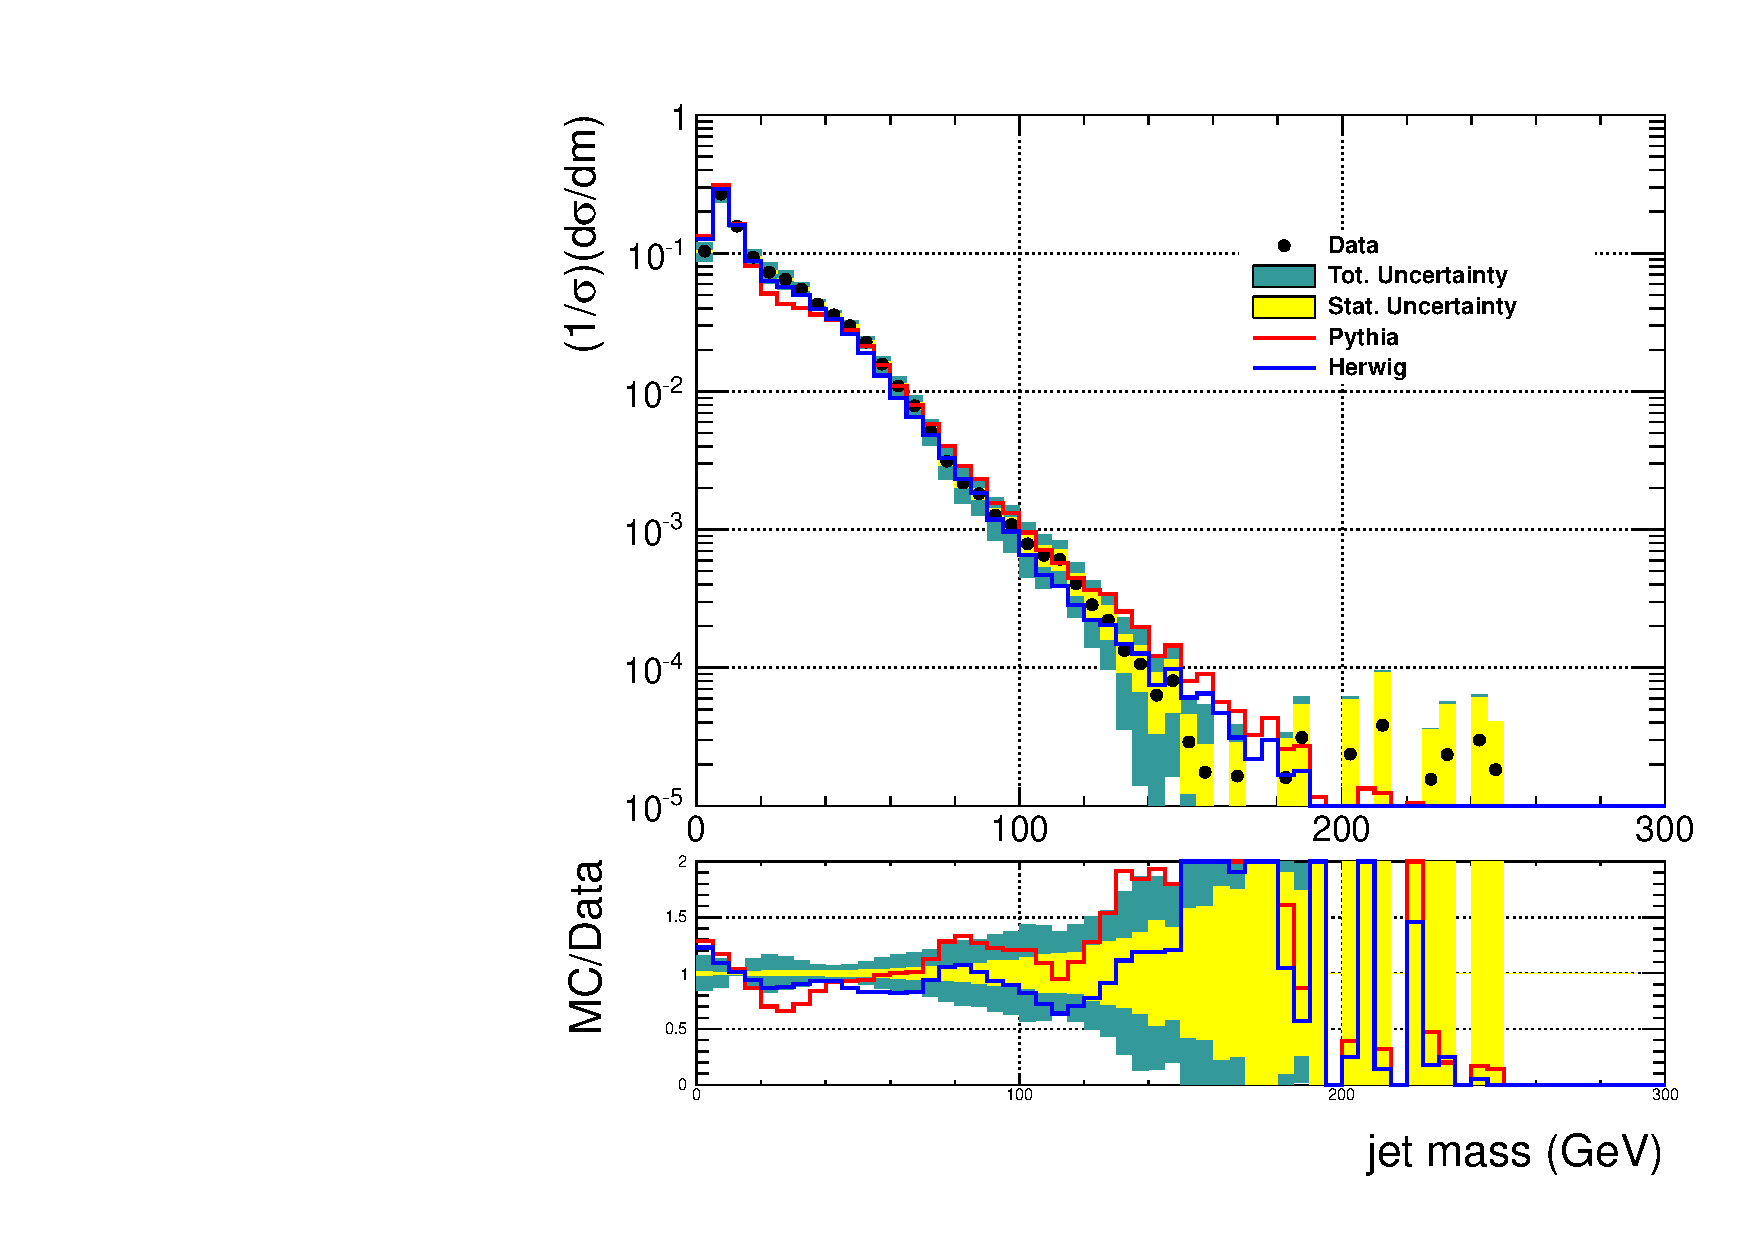
\includegraphics[width=0.49\textwidth]{figs/Wmn/jetmassunf_ak7pr_allpT.pdf}
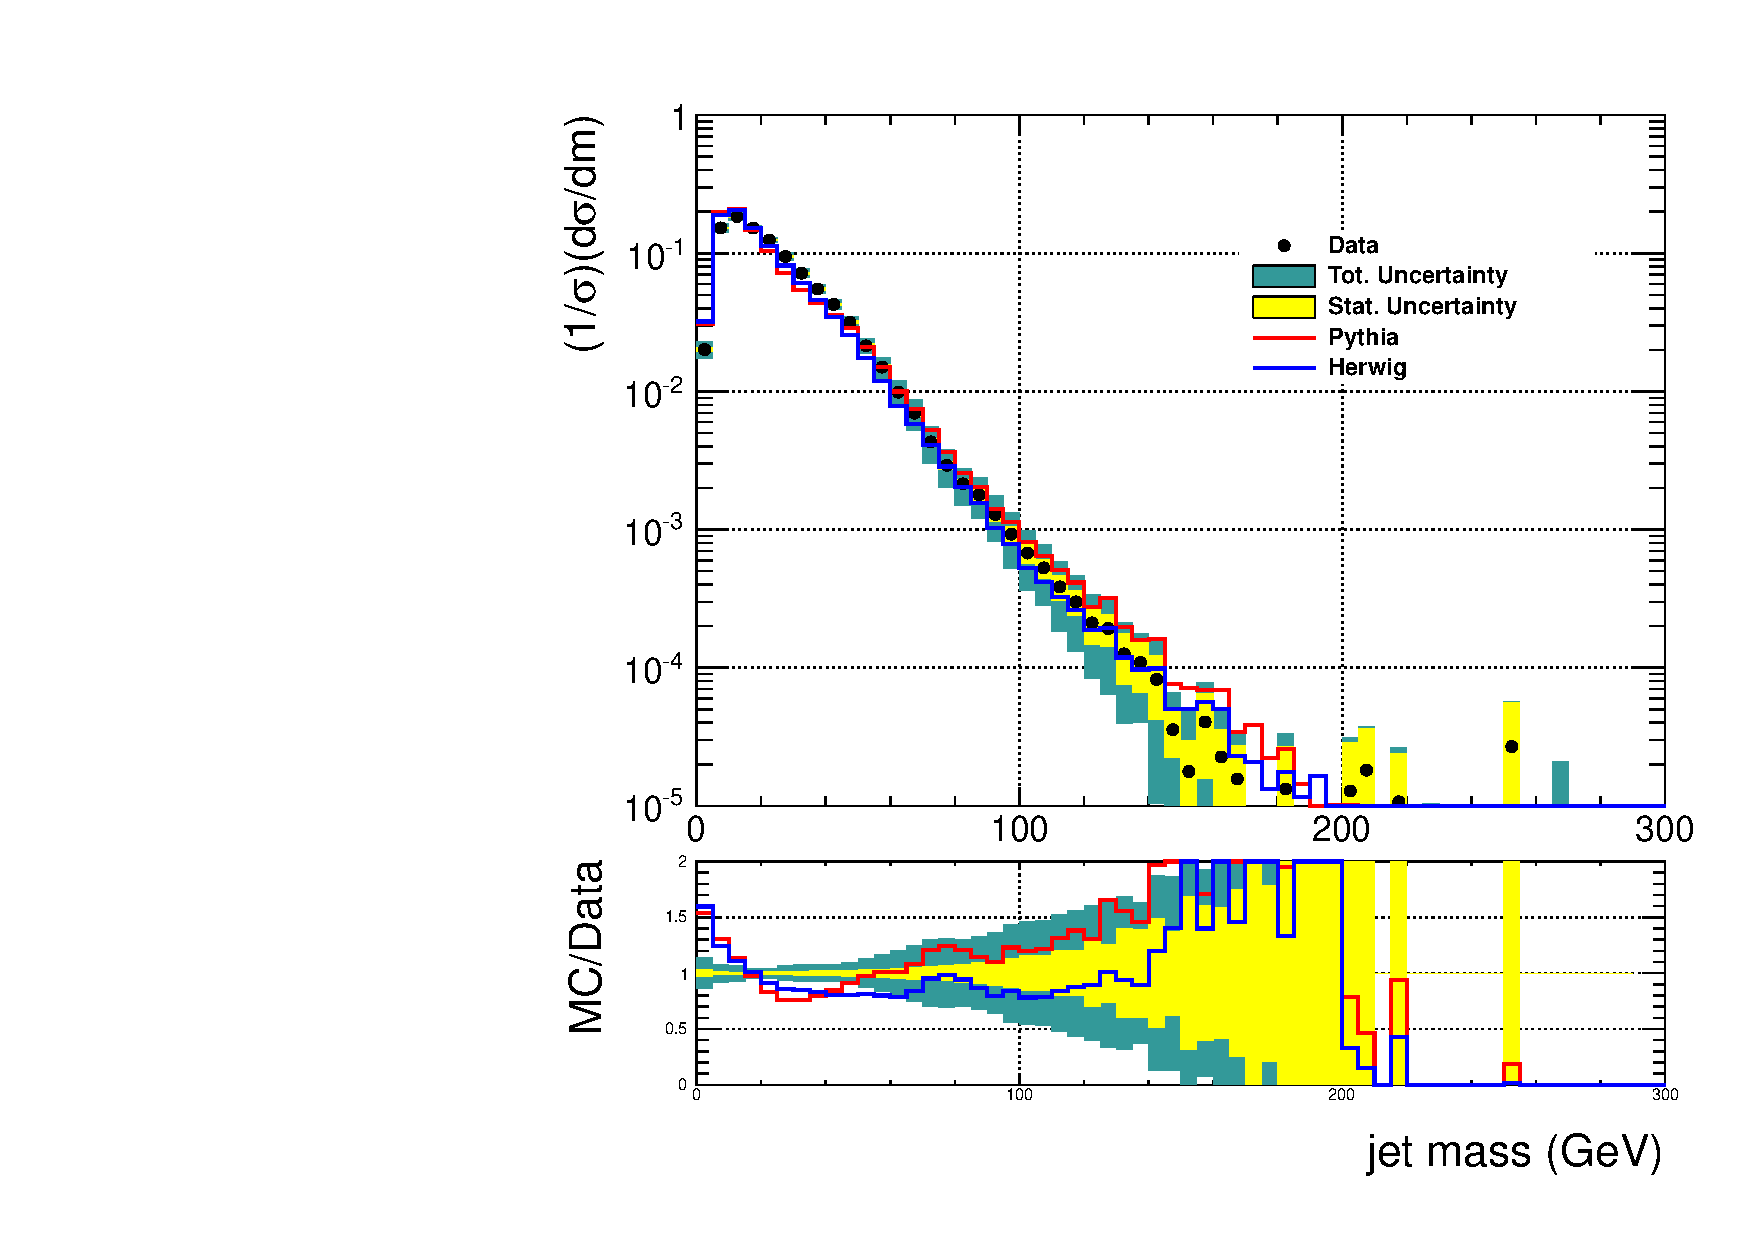
\includegraphics[width=0.49\textwidth]{figs/Wmn/jetmassunf_ak7tr_allpT.pdf}
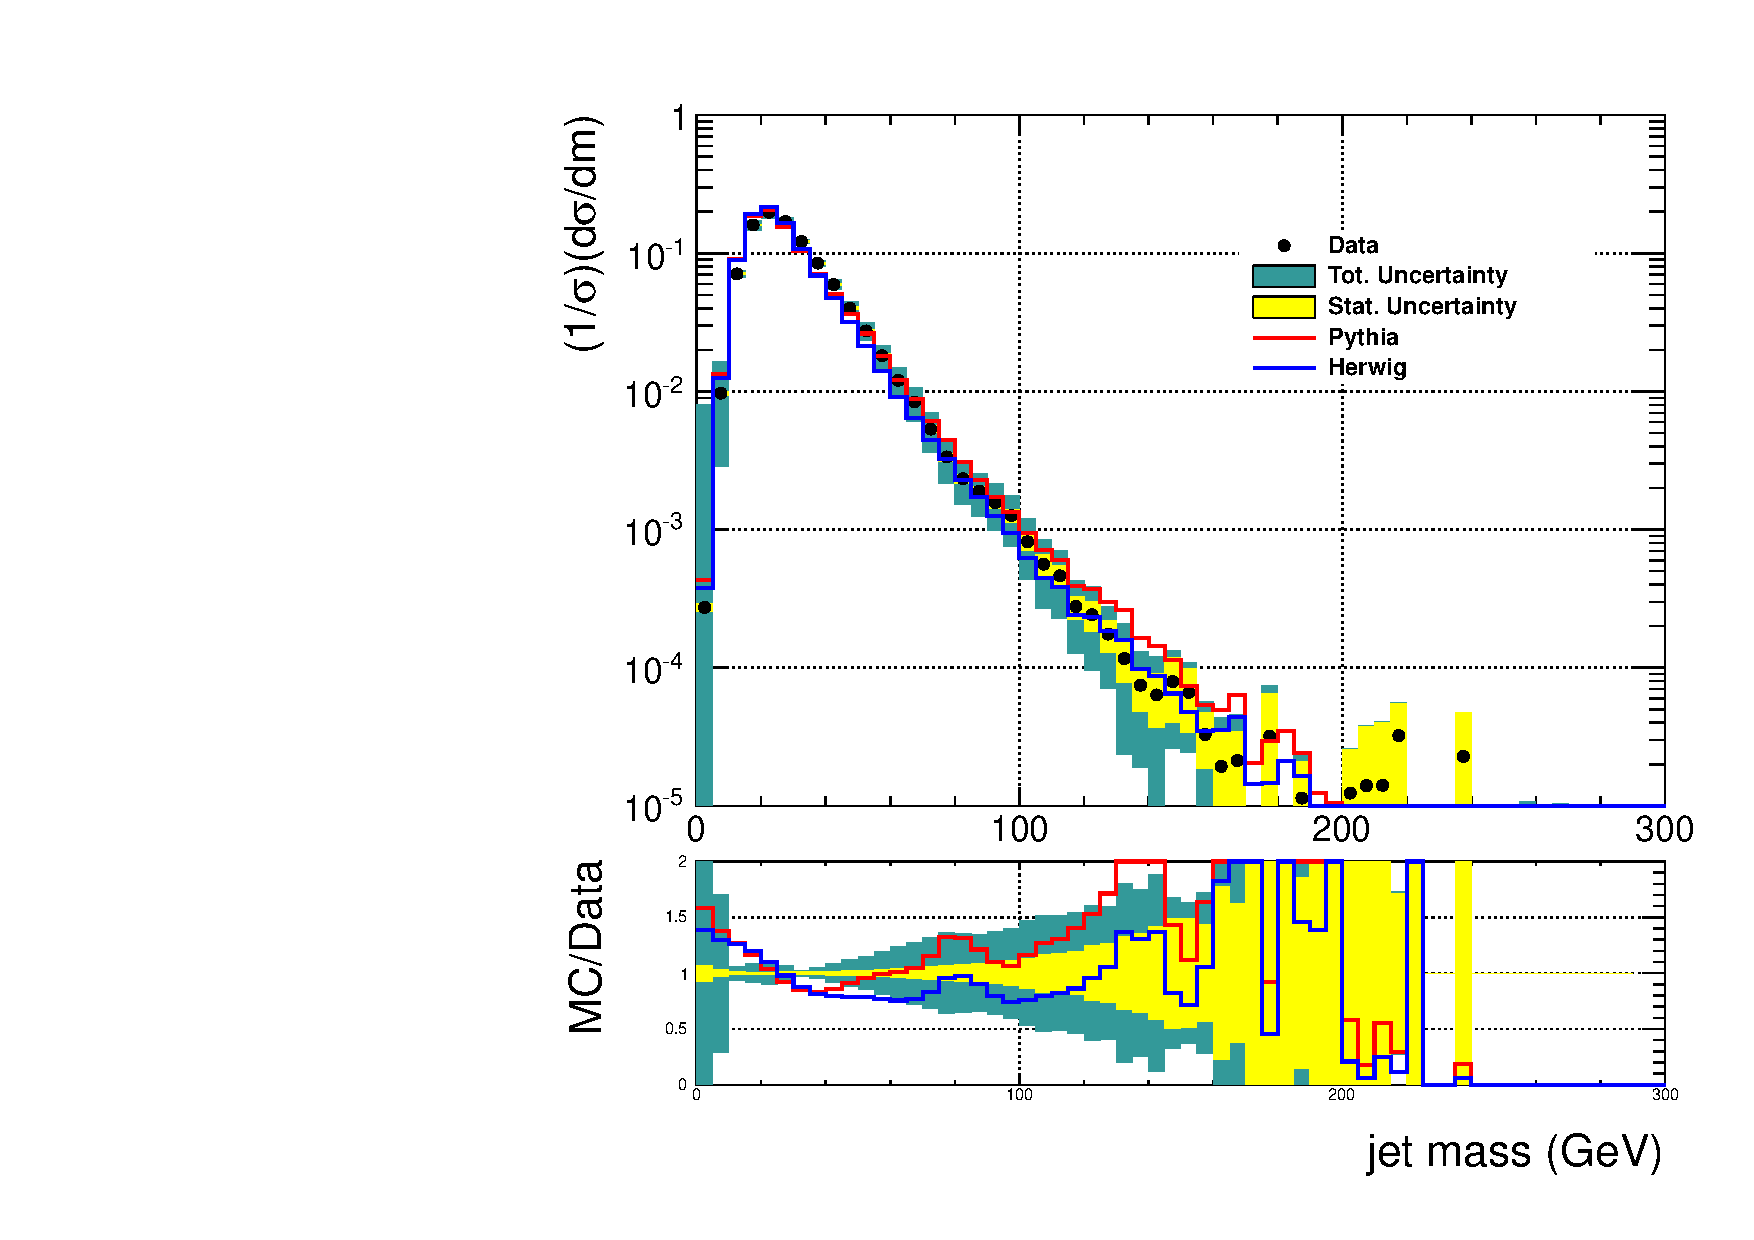
\includegraphics[width=0.49\textwidth]{figs/Wmn/jetmassunf_ak7ft_allpT.pdf}
\caption{Unfolded AK7 ungroomed and groomed jet mass distribution for $W(\mu\nu)$+ jet events. The data (black points) are compared to the MC expectations from Madgraph (solid red) and herwigpp (solid blue). From the top, in clockwise order: ungroomed, pruned, filtered and trimmed jet mass distributions.}
\label{figs:AK7WmnInt1}
\end{figure}


Fig.~\ref{figs:prunedWmnInt1} shows the jet mass distribution for pruned CA 0.8 and filtered CA 1.2 jets in W$(\mu\nu)$ +jet events.

\begin{figure}[!htb]
\centering
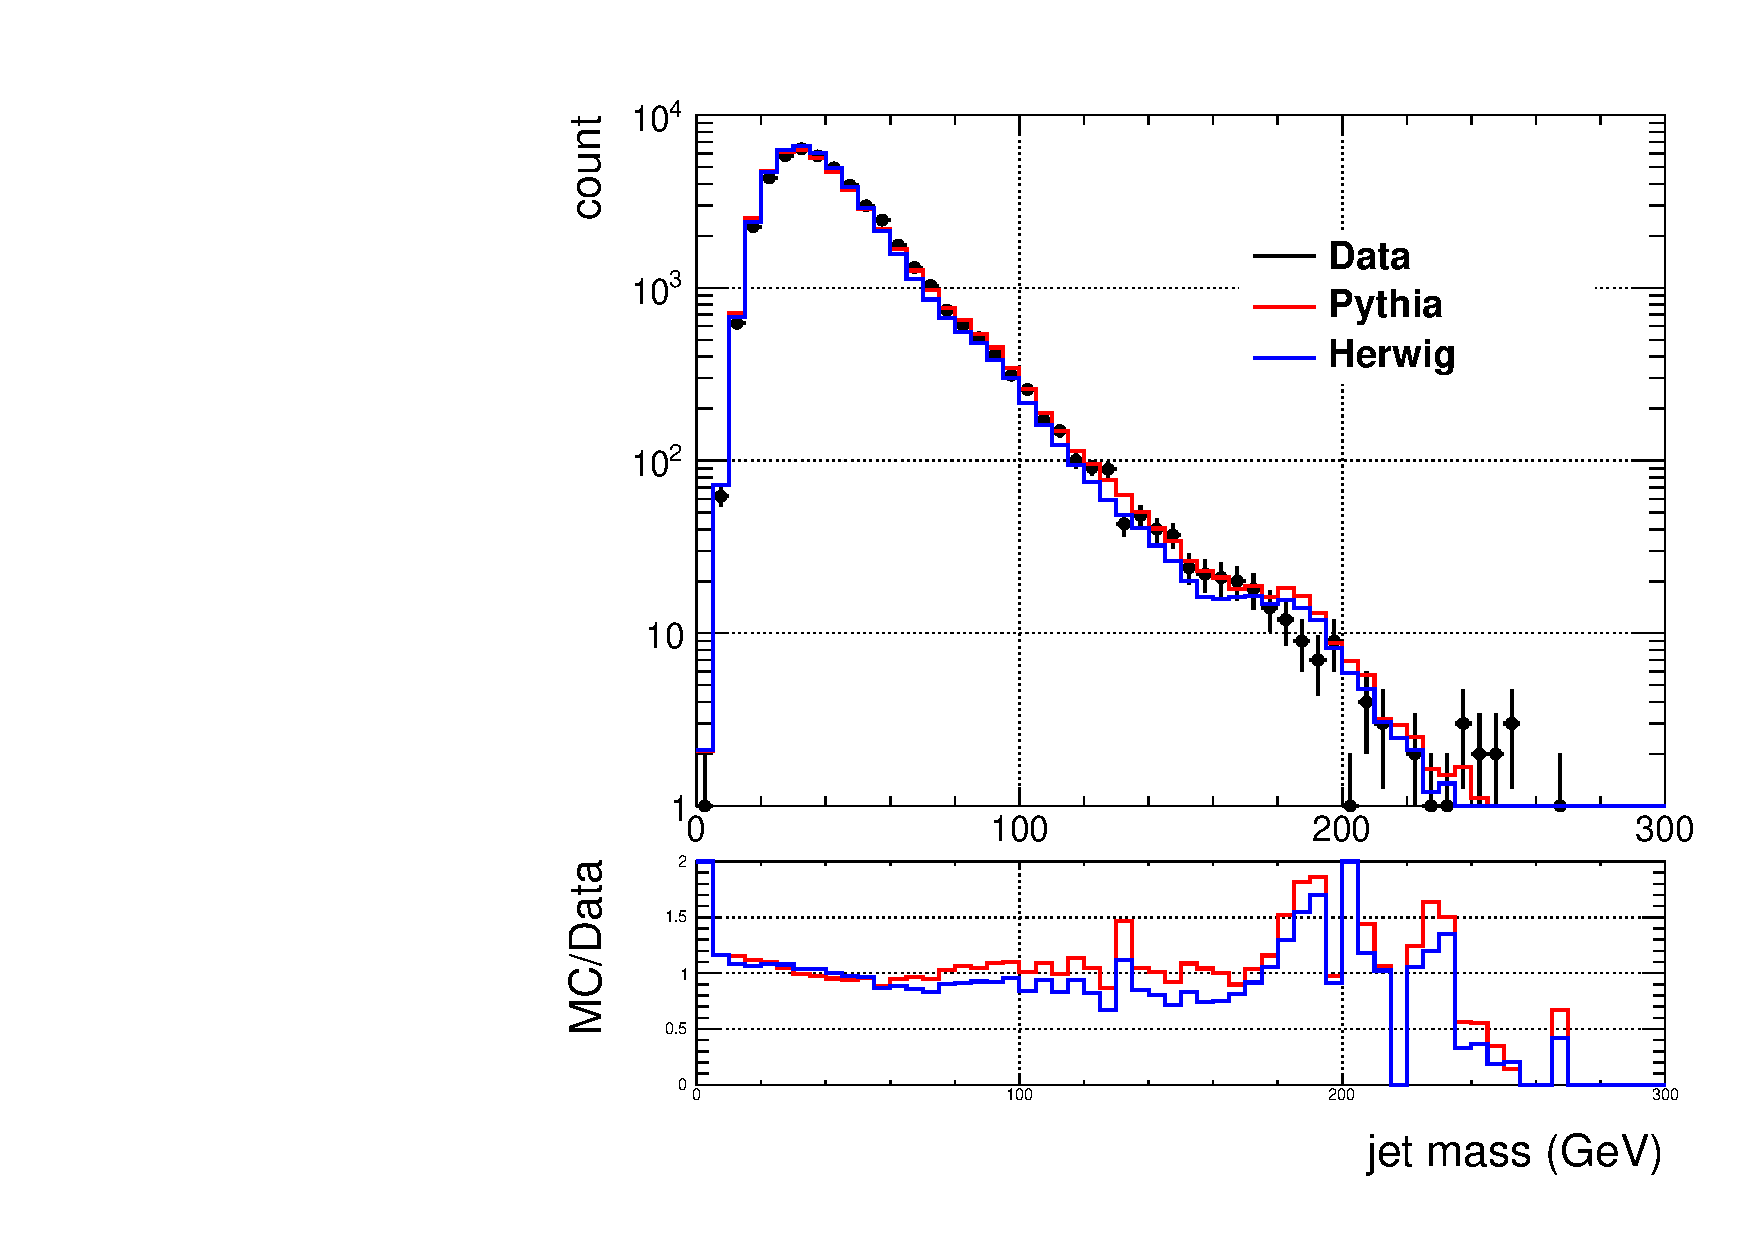
\includegraphics[width=0.49\textwidth]{figs/Wmn/jetmassReco_ca8_allpT.pdf}
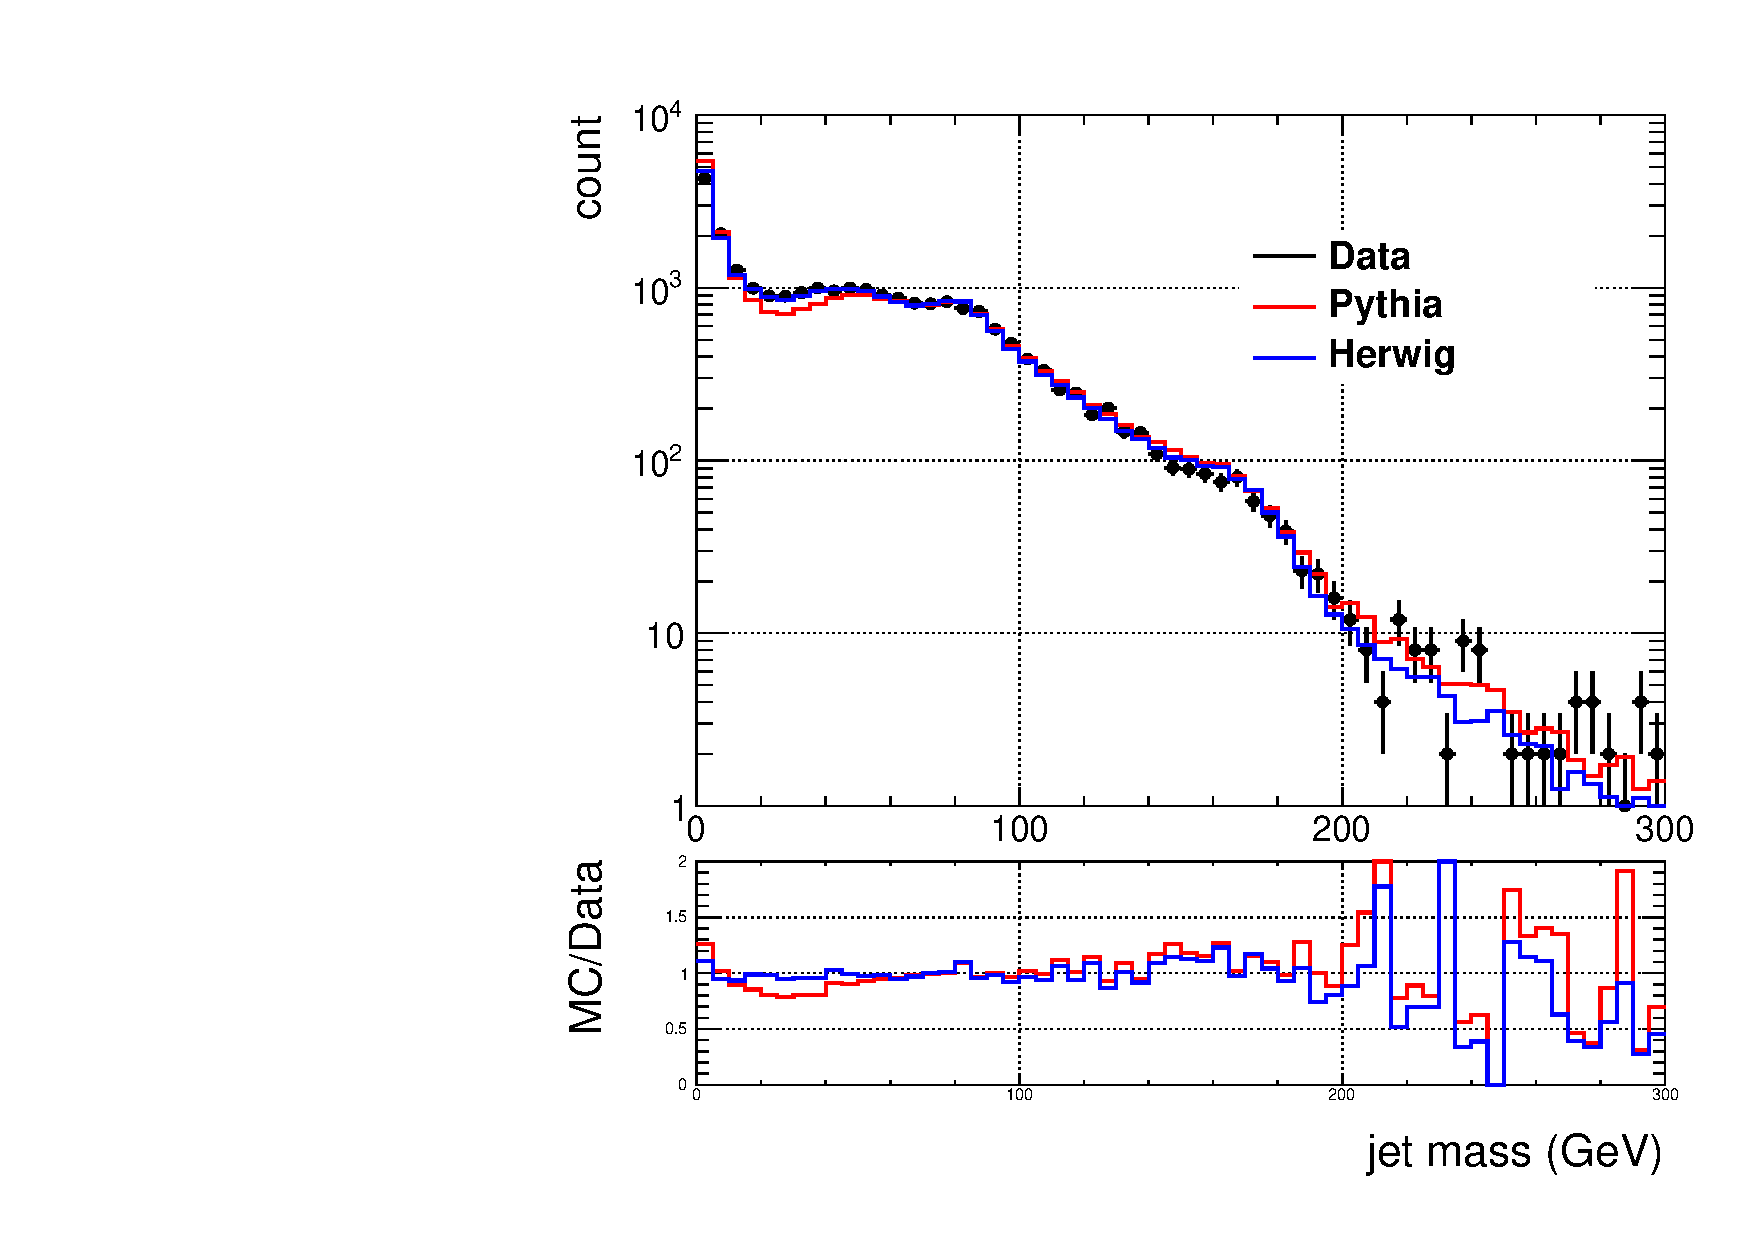
\includegraphics[width=0.49\textwidth]{figs/Wmn/jetmassReco_ca12mdft_allpT.pdf}
\caption{(Not yet Unfolded) CA 0.8 pruned and CA 1.2 filtered jet mass distribution for $W(\mu\nu)$+ jet events. The data (black points) are compared to the MC expectations from Madgraph (solid red) and herwigpp (solid blue).}
\label{figs:prunedWmnInt1}
\end{figure}

\clearpage


\subsection{$W(e\nu)$ + jet Analysis}

Fig.~\ref{figs:AK7WenInt1} shows the jet mass distribution for AK7 jets in W$(e\nu)$ +jet events, for the different clustering algorithm studied: ungroomed, pruned, trimmed and filtered respectively.

\begin{figure}[!htb]\centering
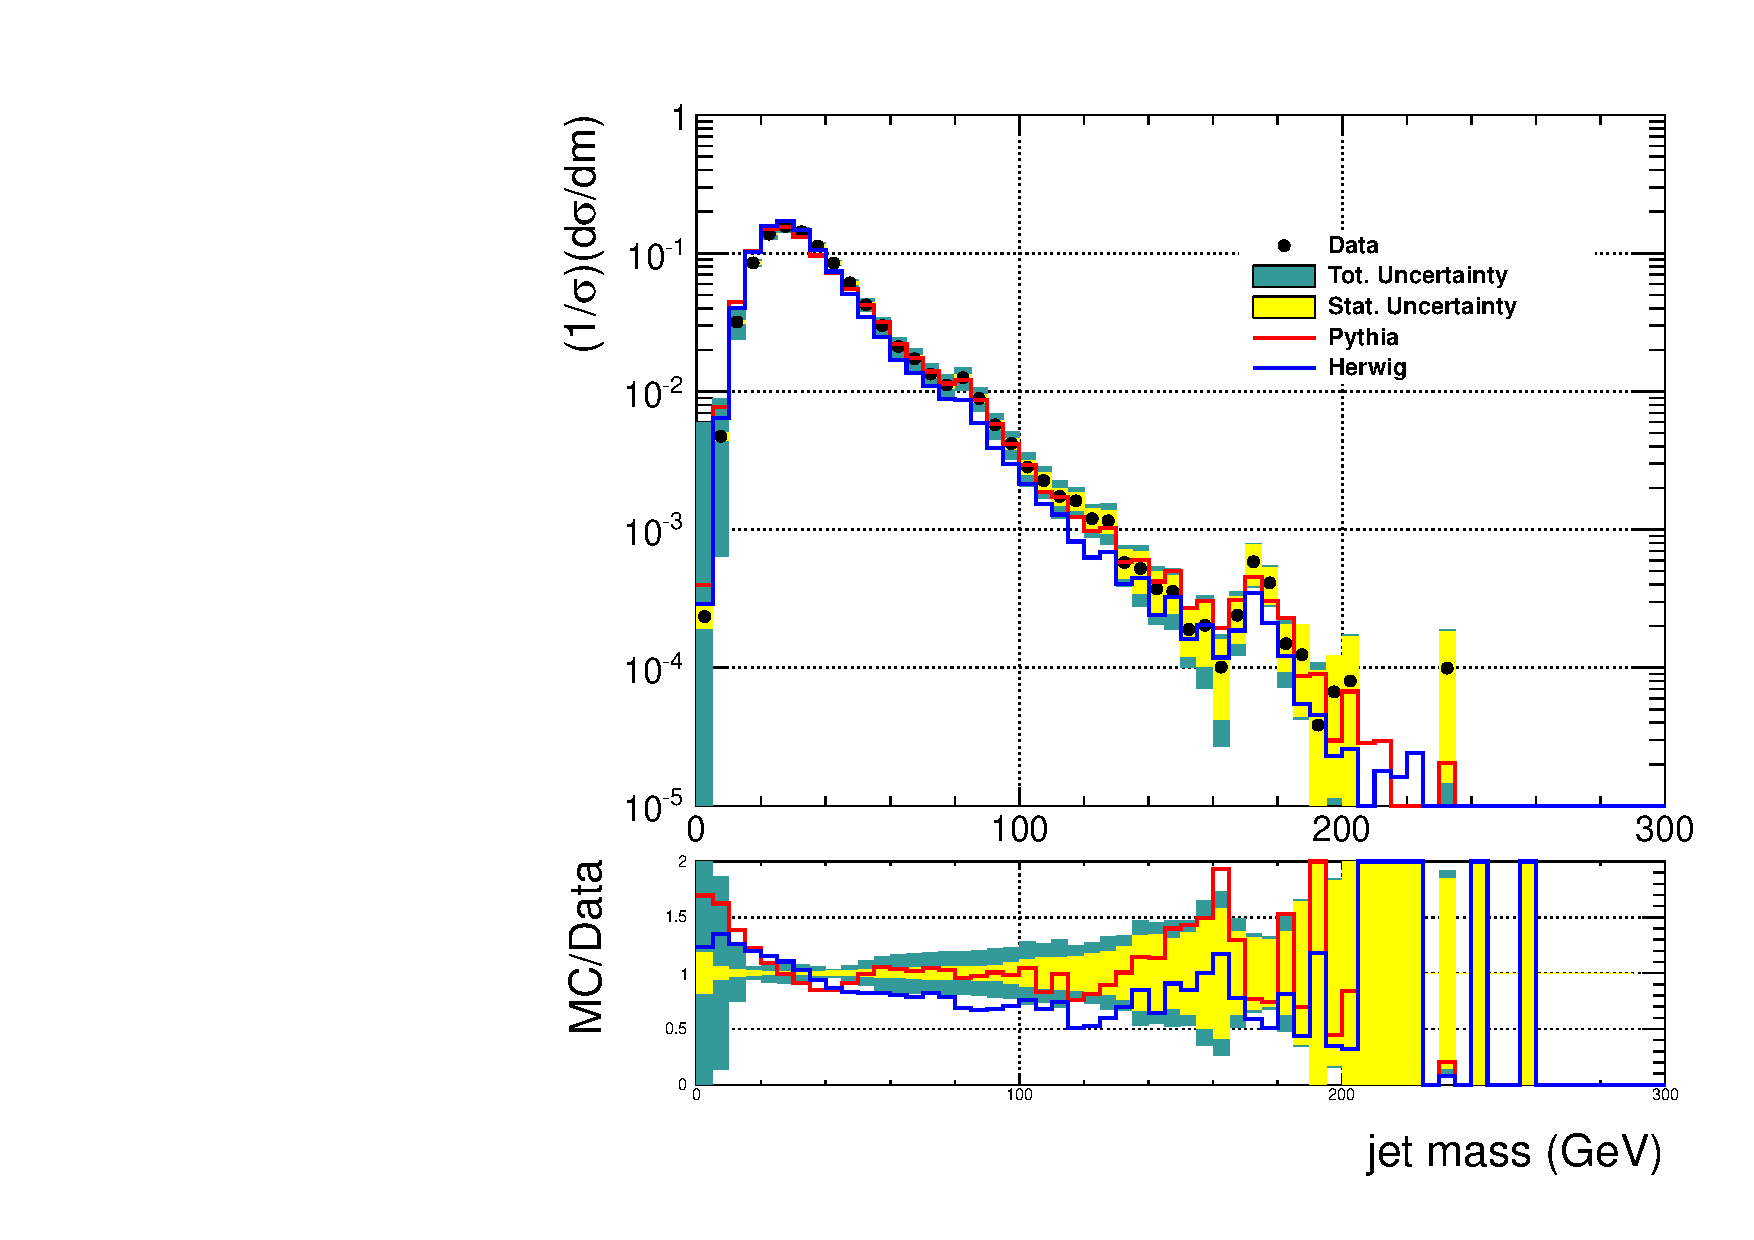
\includegraphics[width=0.49\textwidth]{figs/Wen/jetmassunf_ak7_allpT.pdf}
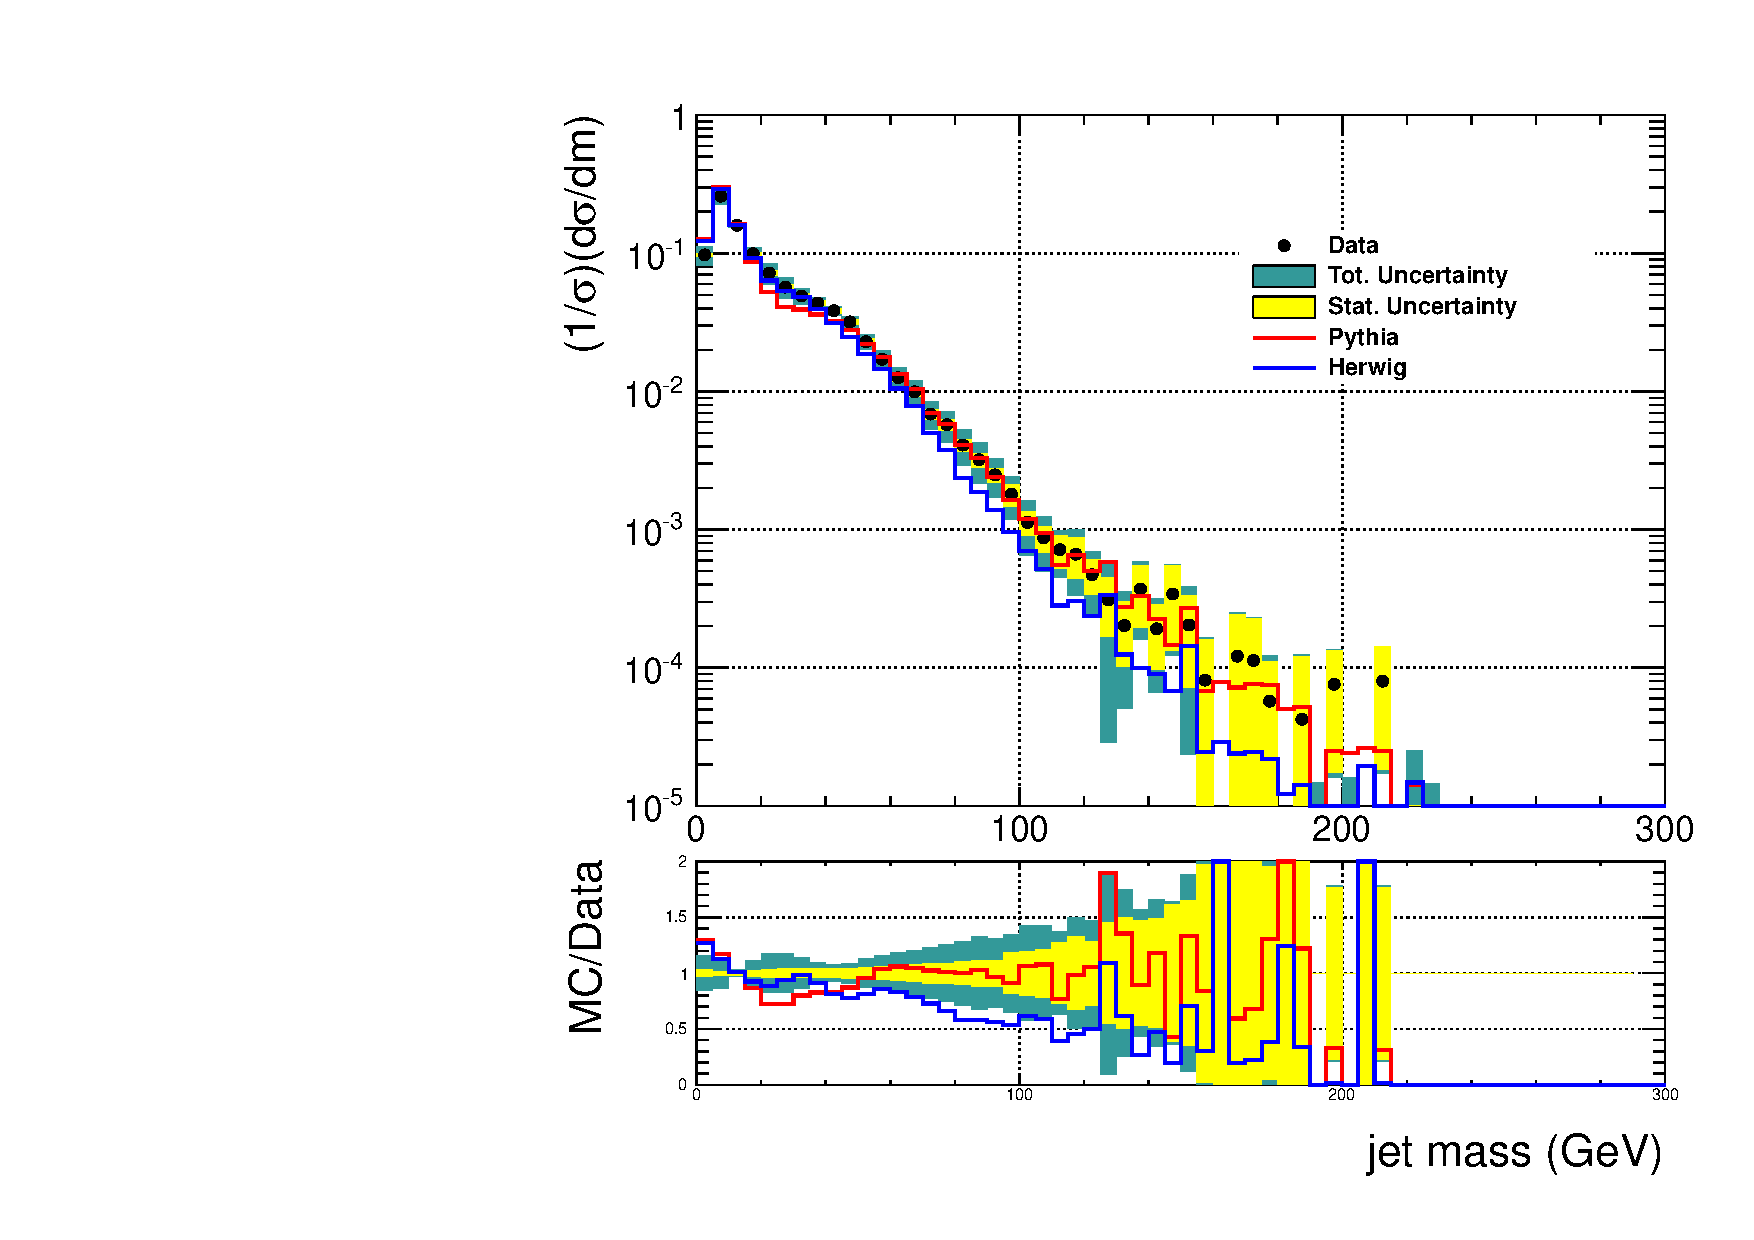
\includegraphics[width=0.49\textwidth]{figs/Wen/jetmassunf_ak7pr_allpT.pdf}
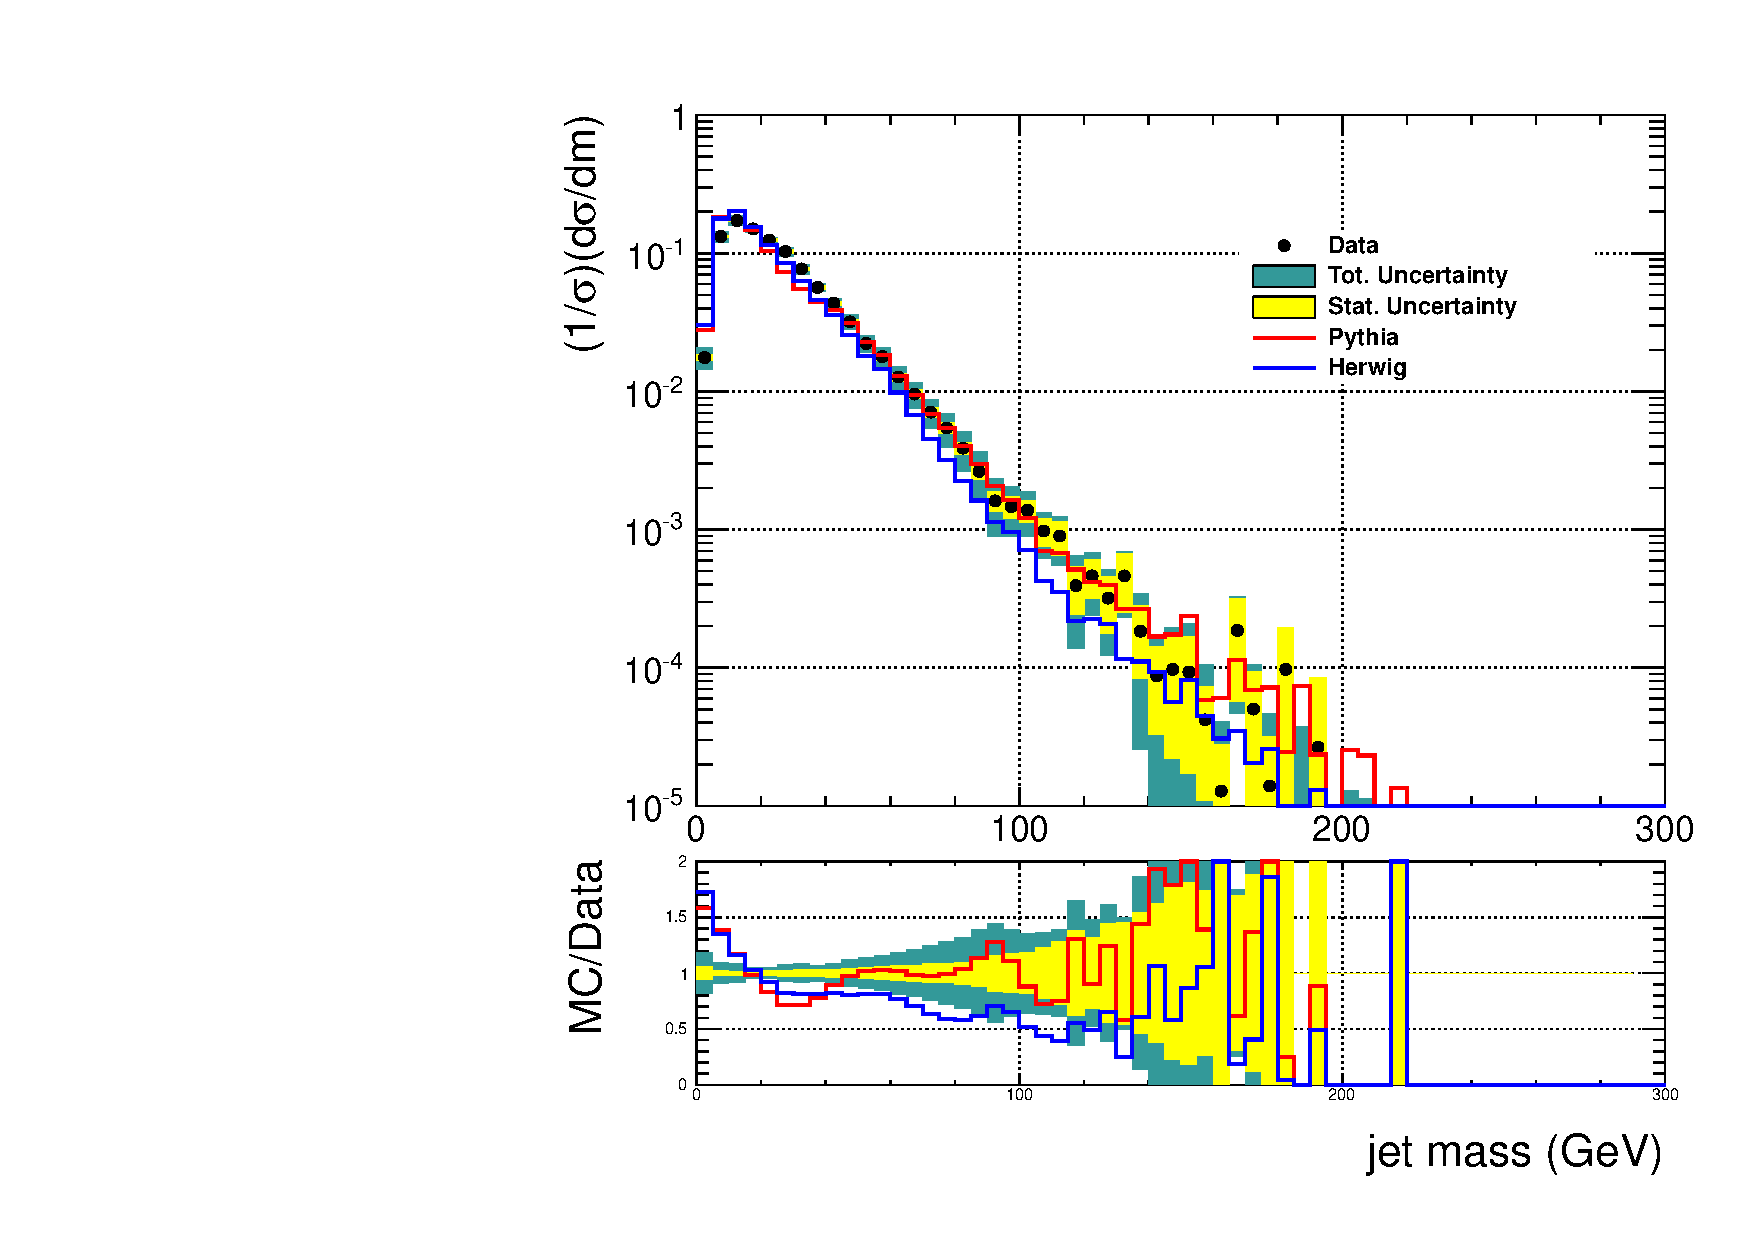
\includegraphics[width=0.49\textwidth]{figs/Wen/jetmassunf_ak7tr_allpT.pdf}
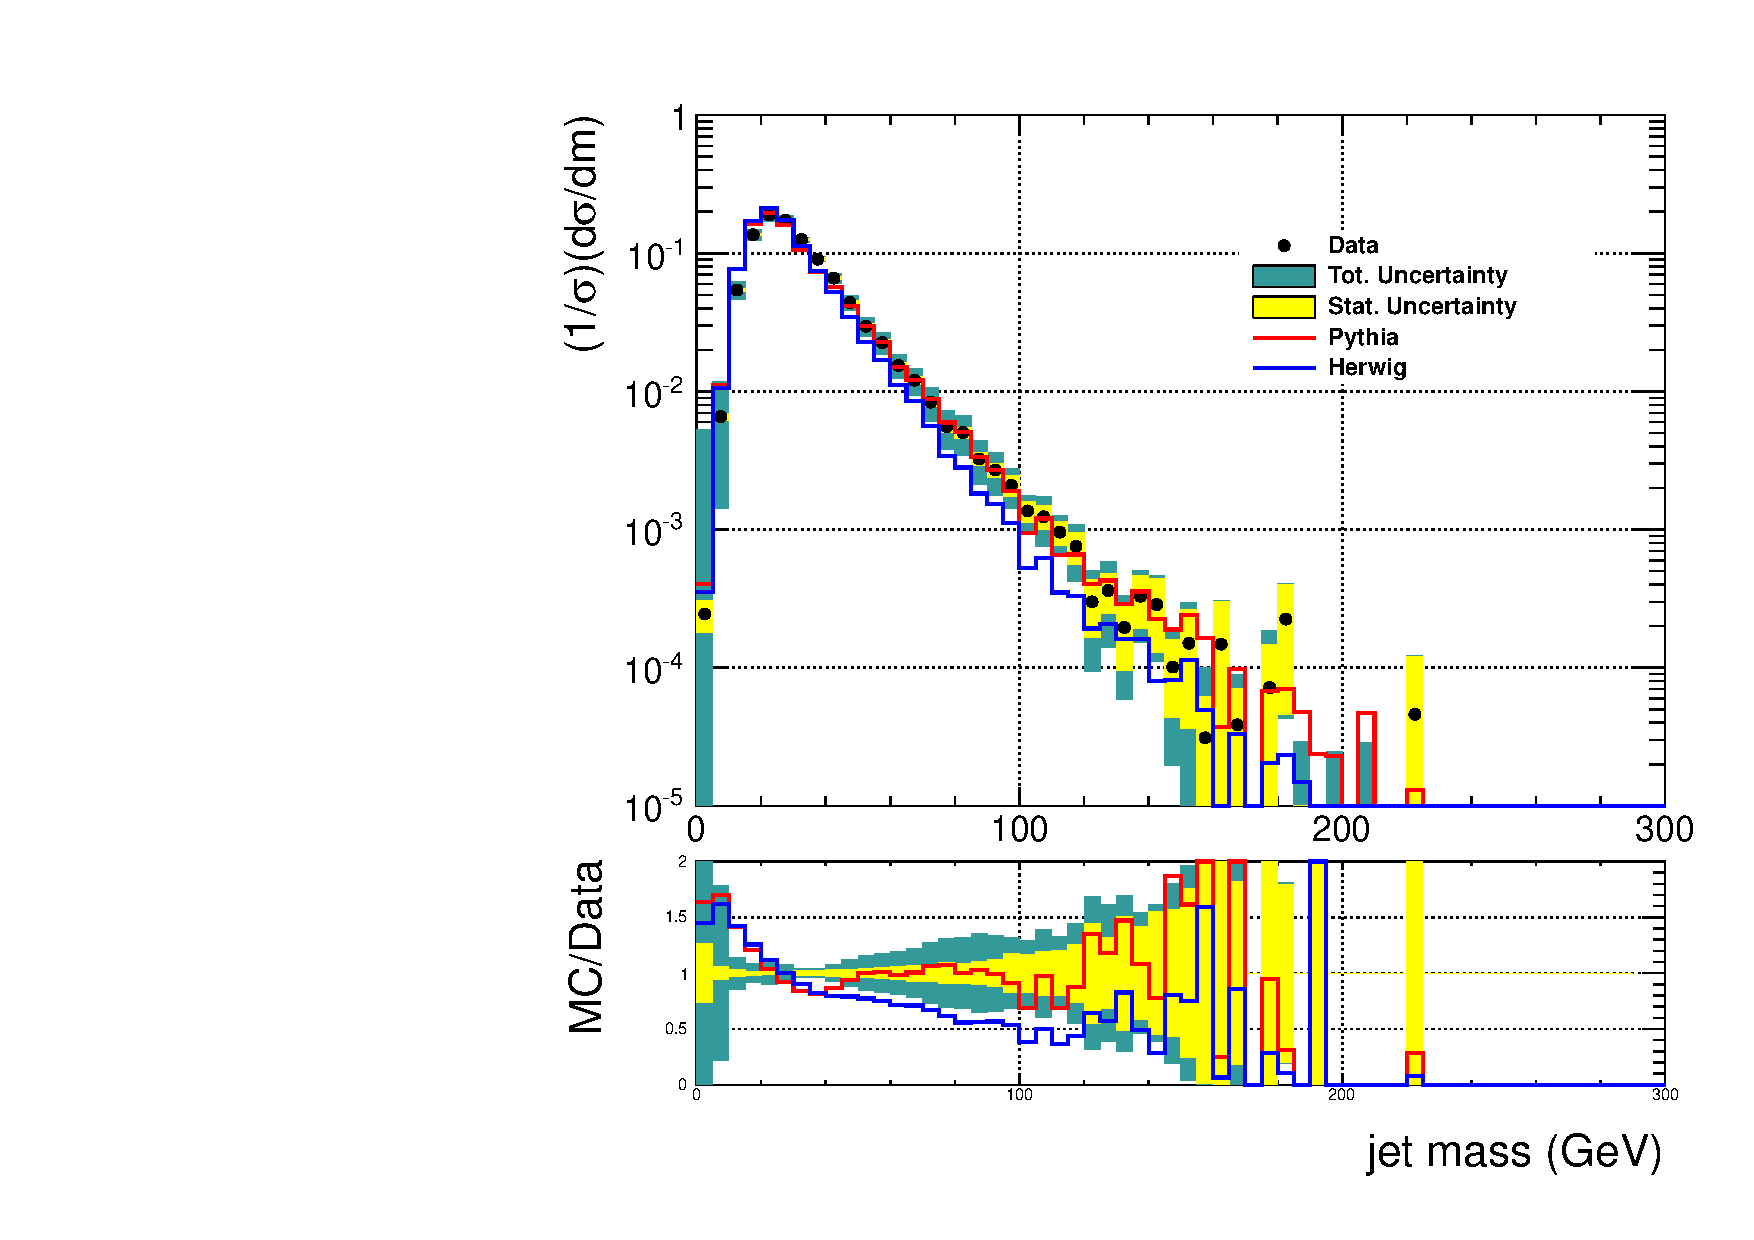
\includegraphics[width=0.49\textwidth]{figs/Wen/jetmassunf_ak7ft_allpT.pdf}
\caption{Unfolded AK7 ungroomed jet mass distribution for $W(e\nu)$+ jet events. The data (black points) are compared to the MC expectations from Madgraph (solid red) and herwigpp (solid blue). From the top, in clockwise order: ungroo
med, pruned, filtered and trimmed jet mass distributions.}
\label{figs:AK7WenInt1}
\end{figure}


Fig.~\ref{figs:prunedWenInt1} shows the jet mass distribution for pruned CA 0.8 and filtered CA 1.2 jets in W$(e\nu)$ +jet events.

\begin{figure}[!htb]
\centering
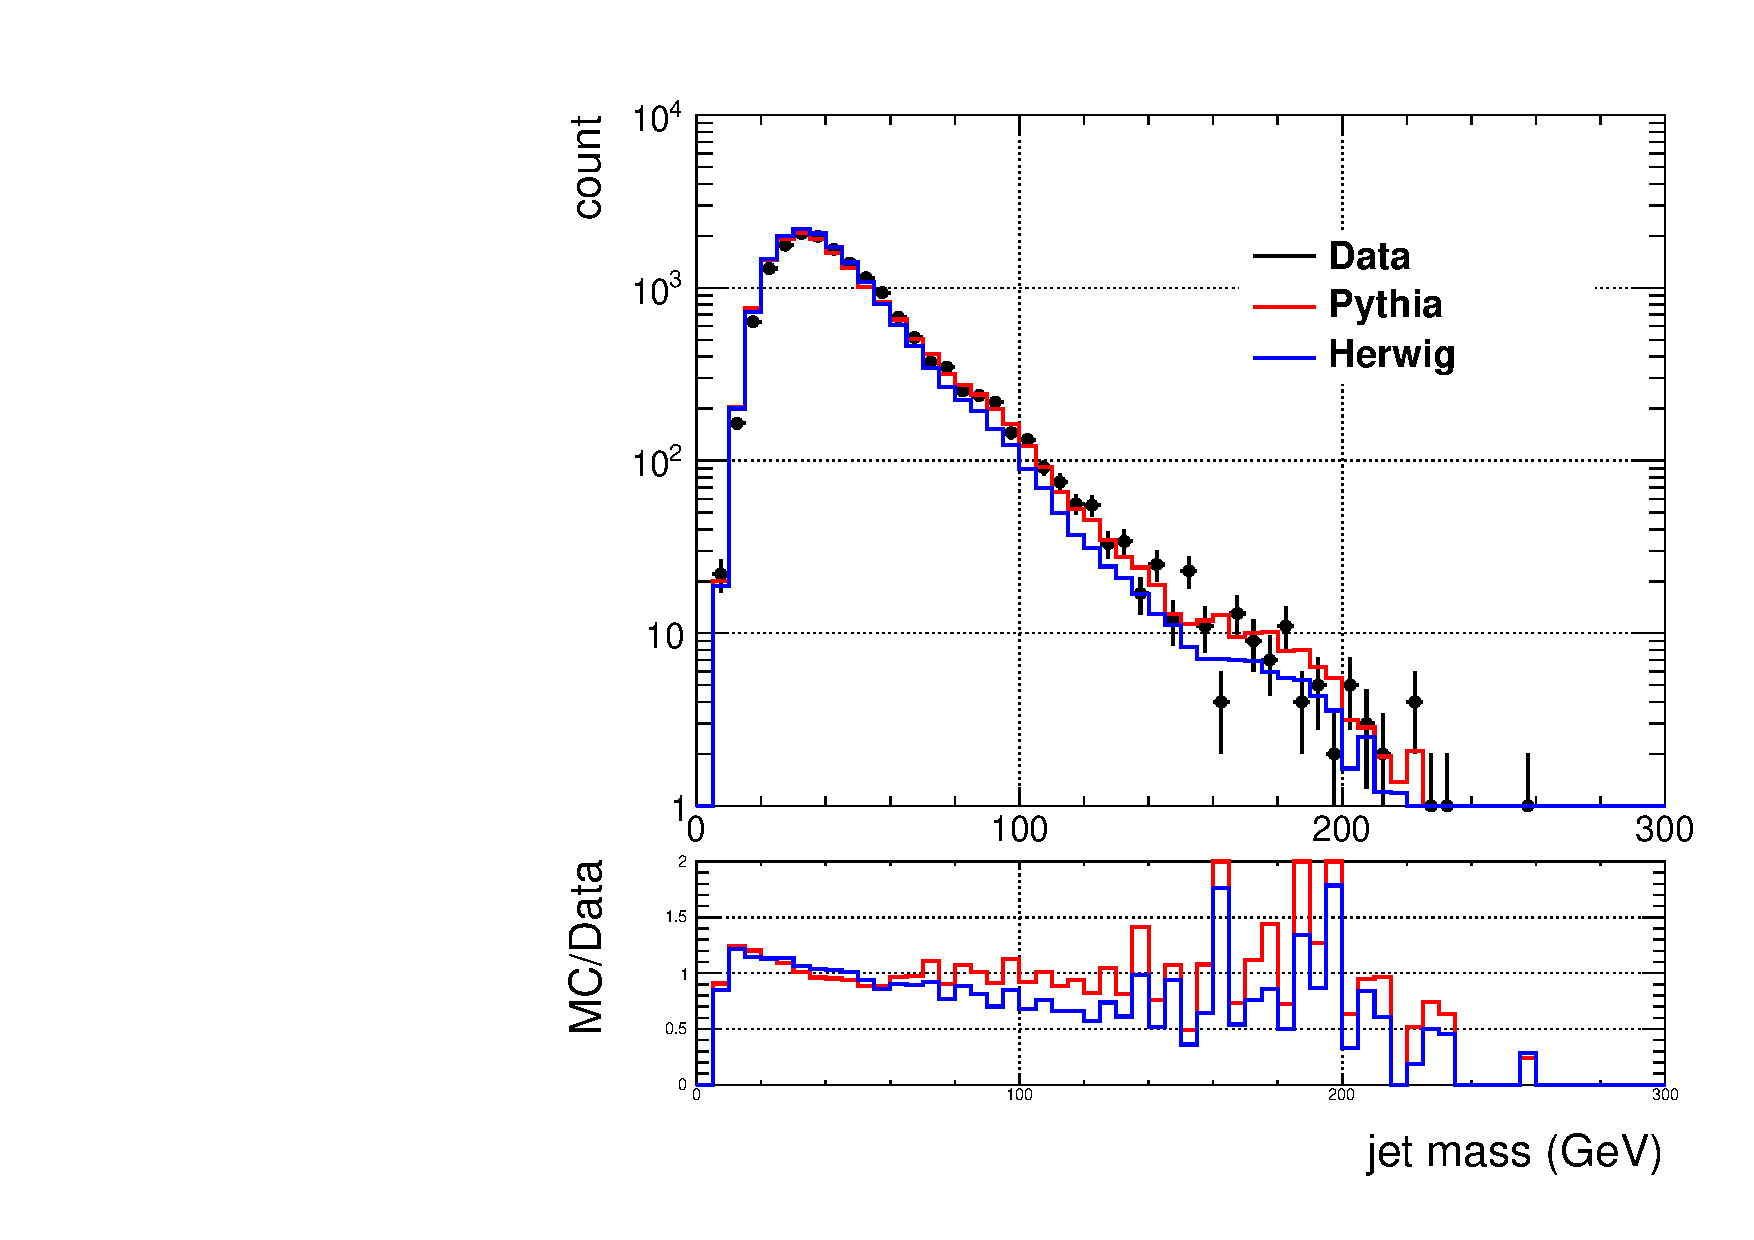
\includegraphics[width=0.49\textwidth]{figs/Wen/jetmassReco_ca8_allpT.pdf}
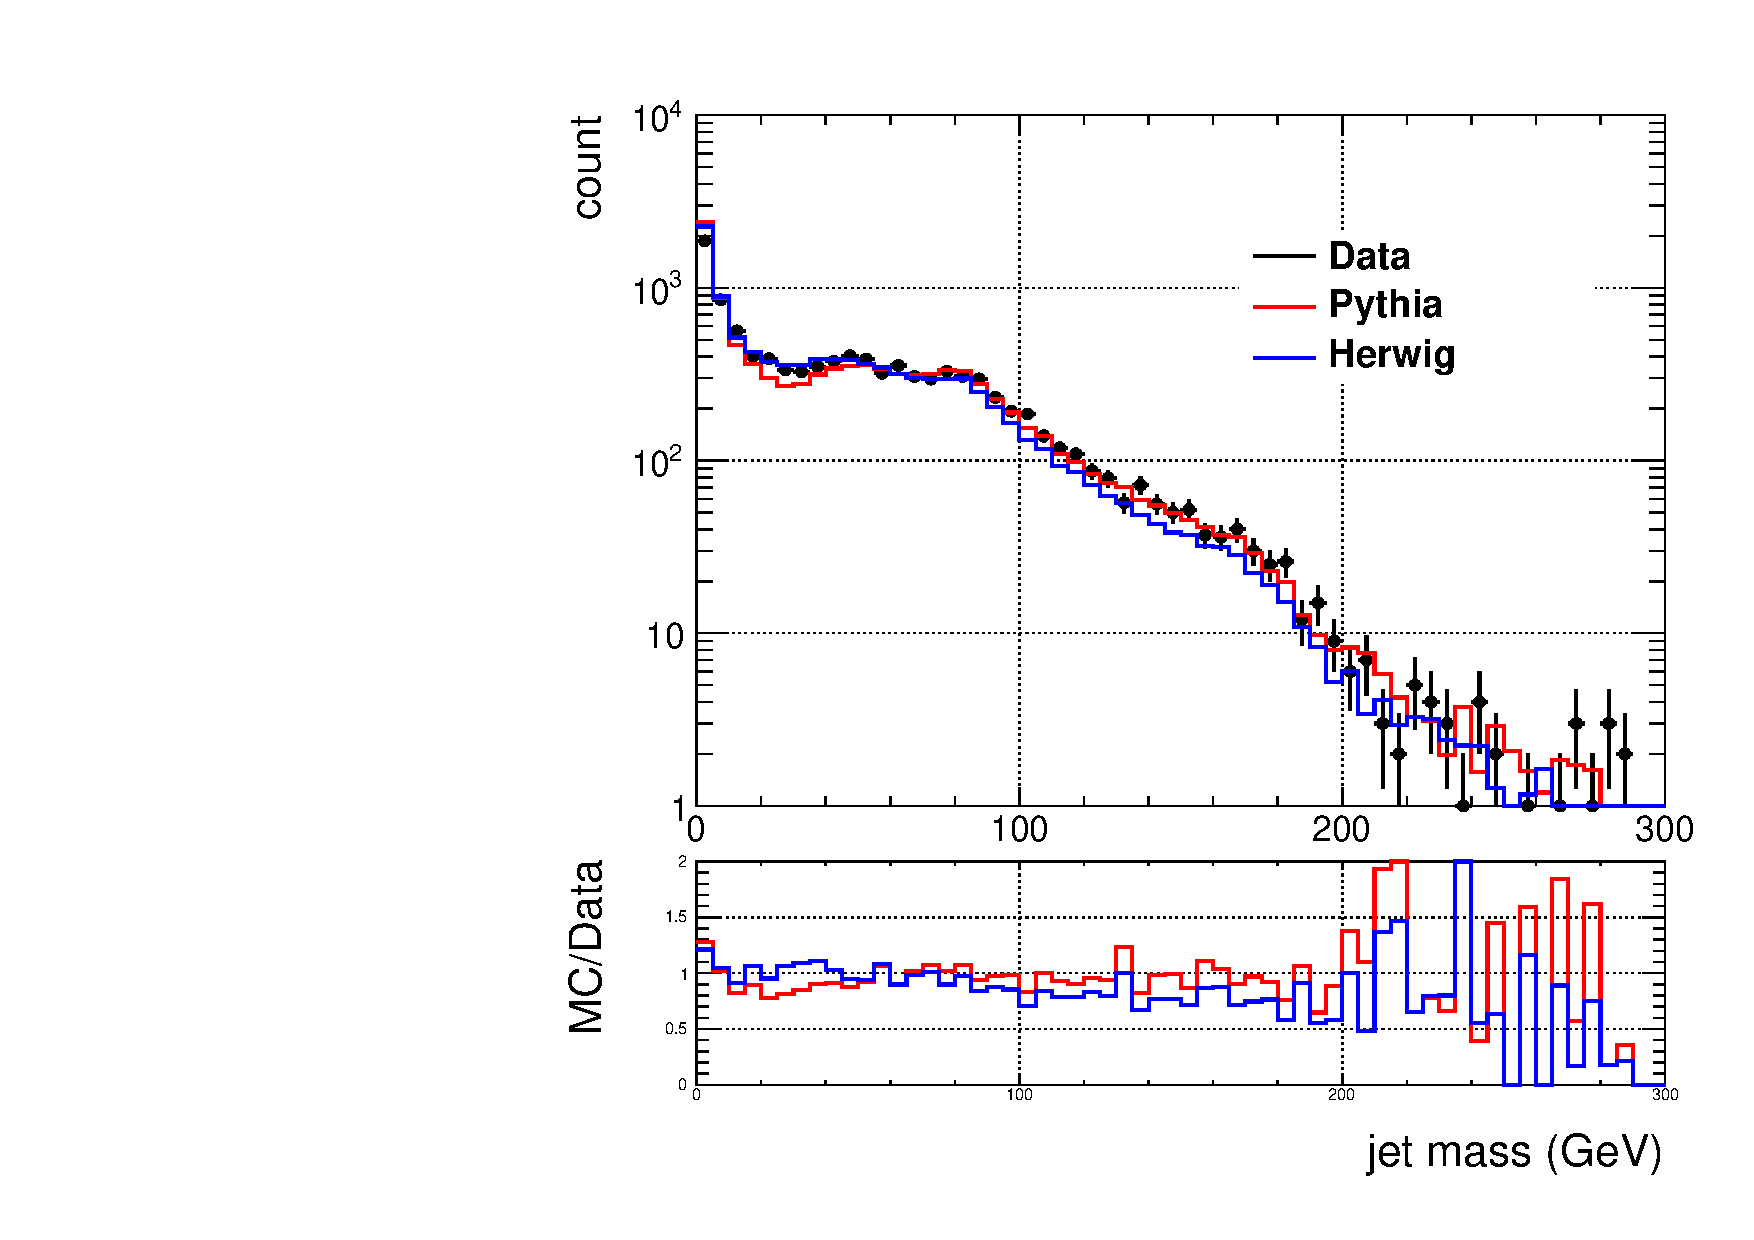
\includegraphics[width=0.49\textwidth]{figs/Wen/jetmassReco_ca12mdft_allpT.pdf}
\caption{(Not yet Unfolded) CA 0.8 pruned and CA 1.2 filtered jet mass distribution for $W(e\nu)$+ jet events. The data (black points) are compared to the MC expectations from Madgraph (solid red) and herwigpp (solid blue).}
\label{figs:prunedWenInt1}
\end{figure}






